\part{Concevoir une \gls{architecture-documentaire} pour les archives historiques de la Faculté de médecine}
\label{part:architecture}

L'histoire, le statut et les conditions de conservation des Archives historiques ayant été établis, reste à déterminer comment en organiser l'accès et la diffusion. Le projet, d'abord envisagé comme un portail réunissant instruments de recherche, informations pratiques, documents numérisés et contenus de valorisation, a rapidement dépassé la conception d'une interface : il faut également déterminer où produire et conserver les descriptions, comment les articuler aux reproductions et comment les signaler au-delà du site de l'Université sans multiplier les saisies.

La réflexion se déplace ainsi de la forme visible du portail vers l'environnement documentaire qui le rend possible. Celui-ci doit distinguer les fonctions, organiser les flux entre les outils et s'inscrire dans les infrastructures comme dans les réseaux de \gls{signalement} auxquels l'Université participe déjà.

Les Archives historiques constituent dès lors un cas d'étude pour la conception d'un environnement consacré à des fonds universitaires patrimoniaux. La démarche consiste à établir les besoins indépendamment d'un logiciel, puis à évaluer les architectures possibles selon leur pertinence documentaire, leur \gls{interoperabilite} et leurs conditions de mise en œuvre.

\chapter{Besoins et conditions d'un environnement documentaire}
\label{chap:besoins}

\section{Un environnement documentaire en cours de structuration}
\label{sec:etat-lieux-documentaire}

\subsection{Des instruments de recherche hétérogènes}

Le futur environnement documentaire devra réunir des descriptions produites au cours de campagnes successives, dont le format, la granularité, le statut, la destination et le degré d'achèvement diffèrent. Le tableau~\ref{tab:etat-instruments-recherche}, sans constituer un état exhaustif des fonds, synthétise les principales situations rencontrées, des instruments publiés aux ensembles encore dépourvus de description exploitable.

\clearpage

\begin{sidewaystable}[p]
	\centering
	\scriptsize
	\setlength{\tabcolsep}{2.5pt}
	\setlength{\arrayrulewidth}{0.4pt}
	\renewcommand{\arraystretch}{0.92}
	
	\begin{tabularx}{0.94\textheight}{
			|>{\raggedright\arraybackslash}p{3cm}
			|>{\raggedright\arraybackslash}p{1.6cm}
			|>{\raggedright\arraybackslash}p{2.1cm}
			|>{\raggedright\arraybackslash}X
			|>{\raggedright\arraybackslash}p{2.5cm}
			|>{\raggedright\arraybackslash}p{2cm}|
		}
		\hline
		\textbf{Ensemble documentaire} &
		\textbf{Cote} &
		\textbf{Dates extrêmes} &
		\textbf{État de la description} &
		\textbf{Instrument disponible} &
		\textbf{Diffusion} \\
		\hline
		
		Fonds ancien
		& A--R et S
		& 1240--1809
		& Classé et décrit ; récolement en cours
		& Inventaire publié par Joseph Calmette
		& Inventaire et registres anciens numérisés dans Foli@ (\texttt{S2}, \texttt{S5}, \texttt{S18}, \texttt{S19} et \texttt{S20}) \\
		\hline
		
		\enquote{Q Supplément}
		& Q+
		& 1532--1987
		& Liste hétérogène ; reclassement nécessaire
		& Cahier manuscrit saisi en 2025
		& Non diffusé en ligne \\
		\hline
		
		Administration générale
		& 1 MED
		& 1794--1981
		& Description en cours de révision et d'harmonisation
		& Répertoire numérique sommaire
		& Site de l'Université \\
		\hline
		
		Enseignement
		& 2 MED
		& 1739--1982
		& Description en cours de révision et d'harmonisation
		& Répertoire numérique détaillé
		& Site de l'Université \\
		\hline
		
		Fonds d'affiches
		& 1 Fi/MED
		& 1852--1985
		& Description révisée et achevée en 2025
		& Répertoire numérique détaillé
		& Site de l'Université \\
		\hline
		
		Registres de scolarité et de gestion des personnels
		& REG
		& An XI--2003
		& Recensement provisoire ; répartition ultérieure dans les instruments correspondants
		& Liste interne numérique et thématique
		& Non diffusée en ligne \\
		\hline
		
		Sous-fonds publics récemment traités
		& LEG, MAIE, PARA, HERB, JM, 1 JDP
		& 1731--2005
		& Descriptions autonomes achevées ou provisoires
		& Répertoires numériques
		& Non diffusés en ligne \\
		\hline
		
		Fonds privés et sociétés savantes traités
		& FB, GG, MG, PB, SMHM, SSMB, 1STE, 2STE
		& 1764--2022
		& Descriptions autonomes disponibles
		& Répertoires numériques
		& Non diffusés en ligne \\
		\hline
		
		Ensembles iconographiques et audiovisuels
		& Fi/GG, AV/GG, 2 Fi/MED
		& 1892--1977
		& Descriptions détaillées disponibles
		& Répertoires numériques
		& Non diffusés en ligne \\
		\hline
		
		Fonds Émile Jeanbrau
		& EJ et 1 EJ
		& 1893--1949
		& Seul le sous-fonds 1 EJ, relatif à la transfusion sanguine, est décrit ; le reste du fonds EJ ne l'est pas
		& Répertoire numérique de 1 EJ
		& Non diffusé en ligne \\
		\hline
		
		Archives modernes non classées
		& Sans cote définitive
		& 1789--2005
		& Non classées et non décrites
		& Aucun instrument de recherche
		& Aucune diffusion \\
		\hline
		
		Fiches et dossiers d'étudiants
		& Sans cote définitive
		& XIX\textsuperscript{e}--XX\textsuperscript{e} siècles
		& Classement matériel alphabétique ou chronologique
		& Outils de repérage matériel uniquement
		& Aucune diffusion \\
		\hline
		
		Dons récemment reçus
		& Sans cote définitive
		& XVIII\textsuperscript{e}--XX\textsuperscript{e} siècles
		& Non traités
		& Aucun instrument de recherche
		& Aucune diffusion \\
		\hline
	\end{tabularx}
	
	\vspace{0.3em}
	
	\begin{minipage}{0.94\textheight}
		\scriptsize
		\emph{Note de lecture :} les termes \enquote{inventaire} et
		\enquote{répertoire} reprennent la dénomination des instruments
		eux-mêmes. Le répertoire numérique présente généralement les
		descriptions dans l'ordre des cotes ; les qualificatifs
		\enquote{sommaire} et \enquote{détaillé} en indiquent le degré de
		précision. Les outils de repérage matériel permettent seulement de
		localiser les documents. Les cotes des instruments non encore
		stabilisés et publiés sont données à titre indicatif et peuvent évoluer.
	\end{minipage}
	
	\captionsetup{
		font=scriptsize,
		skip=3pt,
		width=0.94\textheight
	}
	\caption[État synthétique des principaux ensembles et instruments de recherche]
	{État synthétique du traitement, de la description et de la diffusion des principaux ensembles conservés par les Archives historiques, août 2026.}
	\label{tab:etat-instruments-recherche}
\end{sidewaystable}

\clearpage

Le fonds ancien bénéficie du cadre de classement publié par Joseph Calmette, auquel devront être intégrées les informations issues du récolement en cours et de la reprise de la série dite \enquote{Q Supplément}, sans rompre avec les références existantes\footcite{CalmetteCartulaire1912}\footcite{AHFMQSupplement2025}. Les instruments consacrés aux archives modernes de l'administration générale et de l'enseignement, établis respectivement en 2009 et en 2013, sont en cours de révision et d'harmonisation\footcite{Perroud2009FondsModerne}\footcite{Pin2013Enseignement}.

Les campagnes récentes ont produit des instruments autonomes pour les archives relatives aux legs et aux dons,\footcite{Dikoff2025LegsDons} aux études de maïeutique,\footcite{Bertrand2025Maieutique} aux études paramédicales,\footcite{Bertrand2025Paramedical} au certificat d'herboriste,\footcite{Bertrand2025Herboristes} aux jurys médicaux\footcite{Dikoff2026JurysMedicaux} et au Jardin des plantes,\footcite{Fulbert2025JardinPlantes} ainsi que pour les archives d'Edmond Neyraut retrouvées parmi celles de ce dernier\footcite{Bertrand2025Neyraut}. D'autres concernent les fonds Frédéric Bouisson,\footcite{Dikoff2025Bouisson} Gaston Giraud,\footcite{LethielleuxBertrandDikoff2025Giraud} Marthe Giraud,\footcite{BertrandDikoff2025MartheGiraud} Paul Barjon\footcite{BertrandDikoff2025PaulBarjon} et le sous-fonds 1EJ relatif à la transfusion sanguine d'Émile Jeanbrau\footcite{BertrandDikoff2024Jeanbrau}. Les ensembles iconographiques\footcite{LemetayerEtAl2025IconographieGiraud} et audiovisuels\footcite{Bertrand2025AudiovisuelGiraud} de Gaston Giraud, les portraits de professeurs\footcite{Dikoff2025Portraits} et les fonds de la Société montpelliéraine d'histoire de la médecine,\footcite{Bertrand2025SMHM} de la Société des sciences médicales et biologiques de Montpellier et du Languedoc méditerranéen,\footcite{YriarteBertrandDikoff2025SSMB} de la Société de médecine et de chirurgie pratiques et de la Société médicale d'émulation disposent également d'instruments spécifiques, les deux derniers fonds étant réunis dans un même répertoire\footcite{Bertrand2025SocietesSavantes}.

Cette production reste incomplète : seul le sous-fonds 1EJ est décrit au sein du fonds Émile Jeanbrau et l'inventaire des jurys médicaux demeure provisoire. Les archives modernes non classées, une grande partie des fiches et dossiers d'étudiants ainsi que les dons récemment reçus restent dépourvus d'instruments exploitables.

En l'absence de plan de classement général stabilisé pour les archives publiques modernes et contemporaines, les ensembles cohérents sont décrits séparément avant leur intégration éventuelle dans une organisation plus large. La liste interne des registres modernes et contemporains, intitulée \enquote{REG}, répond ainsi à un besoin immédiat de repérage et de communication ; une fois le plan de classement établi, ses descriptions ont vocation à être réparties dans les instruments correspondant aux ensembles fonctionnels concernés, tandis que la liste initiale subsistera comme outil interne\footcite{Dikoff2024Registres}.

Cette évolution suppose de dissocier l'organisation intellectuelle des fonds de leur cotation matérielle. Une unité peut conserver une cote stable tout en changeant de position dans la hiérarchie descriptive, ce qui évite de multiplier les tables de concordance et de fragiliser les références déjà employées dans les communications, mémoires, thèses et publications scientifiques. Cette logique, proche de celle du répertoire méthodique, organise les descriptions indépendamment de l'ordre des cotes\footcite{PIAFRepertoireMethodique}. Elle permet d'intégrer les documents nouvellement retrouvés ou de déplacer des descriptions sans modifier leurs références matérielles. Le système devra ainsi accompagner les reprises et les accroissements tout en préservant la stabilité des cotes et la hiérarchie qui replace chaque unité dans son contexte documentaire\footcite{ISADG2000}.

Enfin, les instruments existants prennent la forme d'inventaires imprimés, de documents bureautiques, de tableaux de suivi, de saisies de cahiers manuscrits ou de répertoires récents. La création d'un environnement commun ne peut donc se réduire à leur conversion mécanique dans un format unique : elle exige d'identifier les descriptions diffusables ou à reprendre, d'harmoniser les informations, puis de les structurer afin d'assurer leur conservation et leur publication indépendamment des fichiers et dispositifs actuels.

\subsection{Une visibilité numérique existante mais dispersée}

La diffusion numérique des fonds reste fragmentée. Le site institutionnel de l'Université, réalisé sous WordPress, donne accès à trois répertoires PDF autonomes, consultables ou téléchargeables depuis des pages distinctes, mais non interrogeables conjointement : celui de l'administration générale de la Faculté, qui décrit 20,22 mètres linéaires d'archives couvrant la période 1794--1981\footcite{Perroud2009FondsModerne}, celui de l'enseignement, portant sur 11,88 mètres linéaires couvrant la période 1739--1982\footcite{Pin2013Enseignement} et celui du fonds d'affiches, qui recense 658 affiches différentes datées de 1852 à 1985\footcite{PerroudBertrandDikoff2025Affiches}\footcite{UMPatrimoineArchives}.

La documentation disponible est pourtant plus étendue : les instruments consacrés aux fonds privés, aux ensembles iconographiques et audiovisuels ainsi qu'aux sous-fonds publics récemment traités ne sont pas publiés. Certains permettent déjà le repérage et la communication, tandis que d'autres restent provisoires ou doivent être harmonisés. La publication d'un instrument ne reflète donc ni l'importance ni le degré réel de traitement d'un fonds, pas plus que sa présence en ligne ne garantit l'achèvement de sa révision.

La valorisation éditoriale relève d'un autre espace. L'exposition virtuelle \enquote{14--18, Médecine au champ d'honneur}, réalisée sous WordPress à partir d'une exposition physique présentée du 12 septembre au 12 novembre 2014, propose une sélection de documents dans une logique de médiation thématique plutôt que de \gls{signalement} systématique\footcite{UMExpositionMedecine1418}.

Les reproductions numériques forment un troisième ensemble. Foli@, la bibliothèque numérique patrimoniale du \gls{scdi}, donne accès aux deux tomes du \emph{Cartulaire de l'Université de Montpellier}, publiés respectivement sous la direction d'Alexandre Germain\footcite{GermainUniversite1890} et par Joseph Calmette\footcite{CalmetteCartulaire1912}, ainsi qu'au \emph{Liber procuratorum} (\texttt{S2})\footcite{AHFMS2}, au registre des actes de 1423 à 1559 (\texttt{S5})\footcite{AHFMS5}, au cérémonial de l'Université (\texttt{S18})\footcite{AHFMS18} et aux registres de matricules de 1502 à 1561 (\texttt{S19})\footcite{AHFMS19} et de 1562 à 1669 (\texttt{S20})\footcite{AHFMS20}. Ces mises en ligne résultent d'opérations ponctuelles portées par le \gls{scdi}\footnote{Le fonctionnement de ce dispositif sera examiné plus loin.}, et non d'un programme systématique de numérisation des Archives historiques.

Un même fonds peut ainsi être décrit, valorisé et numérisé dans trois espaces différents, sans lien direct entre ces contenus. La présence en ligne ne restitue donc qu'une partie des fonds et du travail de description. Une telle dispersion peut entraver leur utilisation : l'enquête menée par Pascale Bugat, Alain Droguet et Benoît Jégouzo auprès des internautes des Archives départementales du Var montre que les instruments de recherche et les informations pratiques figuraient sur le site institutionnel, tandis que les documents numérisés et les bases documentaires relevaient d'un autre espace. La faible circulation entre les deux a conduit le service à renforcer leurs liens et à rendre les inventaires directement accessibles depuis l'interface de consultation\footcite[pp.~154--157]{BugatDroguetJegouzo2007}.

Cette fragmentation rejoint les \enquote{angles morts} de la diffusion archivistique définis par Lydiane Gueit-Montchal : l'usager doit pouvoir distinguer ce qui est décrit de ce qui ne l'est pas, ce qui est accessible en ligne de ce qui ne peut être consulté qu'en salle de lecture et, plus largement, ce qui existe indépendamment de sa présence sur le web. Une ressource absente en ligne risque d'être tenue pour inexistante, tandis que les documents numérisés peuvent occulter les ensembles seulement décrits ou non diffusés numériquement\footcite[p.~14]{GueitMontchal2021}.

Le futur dispositif devra donc rendre visibles les fonds quel que soit leur degré de traitement et relier instruments, contenus éditoriaux et reproductions. Leur réunion sous une même interface ne suffira toutefois pas : les descriptions devront pouvoir être actualisées et réutilisées dans plusieurs environnements sans créer de versions concurrentes.

\subsection{Les usages observés et les besoins d'accès aux fonds}
\label{subsec:acces-documents-fonds}

\paragraph{Un repérage documentaire encore largement assuré par le service}

Les modalités actuelles de diffusion ne renseignent qu'imparfaitement sur les parcours réels des usagers. L'analyse des 152 demandes reçues entre 2024 et 2026 permet néanmoins d'identifier la manière dont elles sont formulées et les recherches auxquelles elles répondent. Les données de 2026 prises en compte dans ces statistiques sont arrêtées à la mi-juillet, date d'achèvement de la collecte menée pour le présent mémoire.

Trois dimensions ont été distinguées. Le \enquote{point d'entrée} correspond aux informations dont dispose initialement le demandeur : nom de personne, repère chronologique, sujet, groupe étudié ou référence archivistique. L'\enquote{objet} désigne les informations recherchées dans les documents. La \enquote{finalité} indique l'usage auquel la recherche est destinée. Ces catégories peuvent donc se combiner : une personne qui cherche à reconstituer les études d'un ancêtre formule une recherche dont le point d'entrée est un nom ou une date, dont l'objet relève de la scolarité et des parcours universitaires et dont la finalité est familiale ou généalogique.

La catégorie \enquote{scolarité et parcours universitaires} rassemble ainsi les recherches portant sur les inscriptions, les études suivies, les examens, les résultats, les diplômes ou le déroulement d'un cursus. Elle se distingue de la catégorie \enquote{vie et carrière d'une personne}, qui concerne plus largement les activités, les fonctions et la trajectoire biographique d'un individu au-delà de ses seules études. Le \enquote{gouvernement et l'histoire institutionnelle} recouvrent les statuts, l'organisation administrative, les instances de décision et les transformations de la Faculté. Les \enquote{enseignements, pratiques et savoirs médicaux} concernent le contenu et l'organisation des cours, les disciplines, les pratiques professionnelles et la production des connaissances. Enfin, la catégorie \enquote{patrimoine, bâtiments et collections} réunit les recherches relatives aux édifices ainsi qu'à la constitution, à la conservation et à la valorisation des collections archivistiques, bibliographiques, scientifiques ou artistiques.

La finalité \enquote{recherche familiale ou généalogique} ne définit donc pas le contenu des documents recherchés, mais l'usage qui en sera fait : elle correspond aux demandes visant à documenter un ascendant, un parent ou une histoire familiale. Elle peut porter sur la scolarité d'une personne comme sur sa carrière ou sur tout autre aspect de sa vie. La \enquote{recherche universitaire} s'inscrit dans un travail académique ; la \enquote{recherche personnelle ou érudite} est conduite hors de ce cadre ; les projets de \enquote{valorisation ou de médiation} visent notamment une exposition, une publication ou un contenu culturel ; les besoins \enquote{professionnels ou institutionnels} répondent au fonctionnement d'un service ou d'un organisme.

Sur les 152 demandes étudiées, 102, soit 67,1\,\%, prennent pour point d'entrée un nom de personne ou un repère chronologique ; 29, soit 19,1\,\%, un sujet de recherche ; et six, soit 3,9\,\%, un groupe de personnes étudié. À l'inverse, huit seulement, soit 5,3\,\%, mentionnent d'emblée un document ou une cote déjà identifiés et six, soit 3,9\,\%, un fonds ou une série déjà identifiés. Une demande demeure indéterminée. Au total, seules 14 demandes, soit 9,2\,\%, comportent donc une référence archivistique préalablement identifiée.

\begin{figure}[htbp]
	\centering
	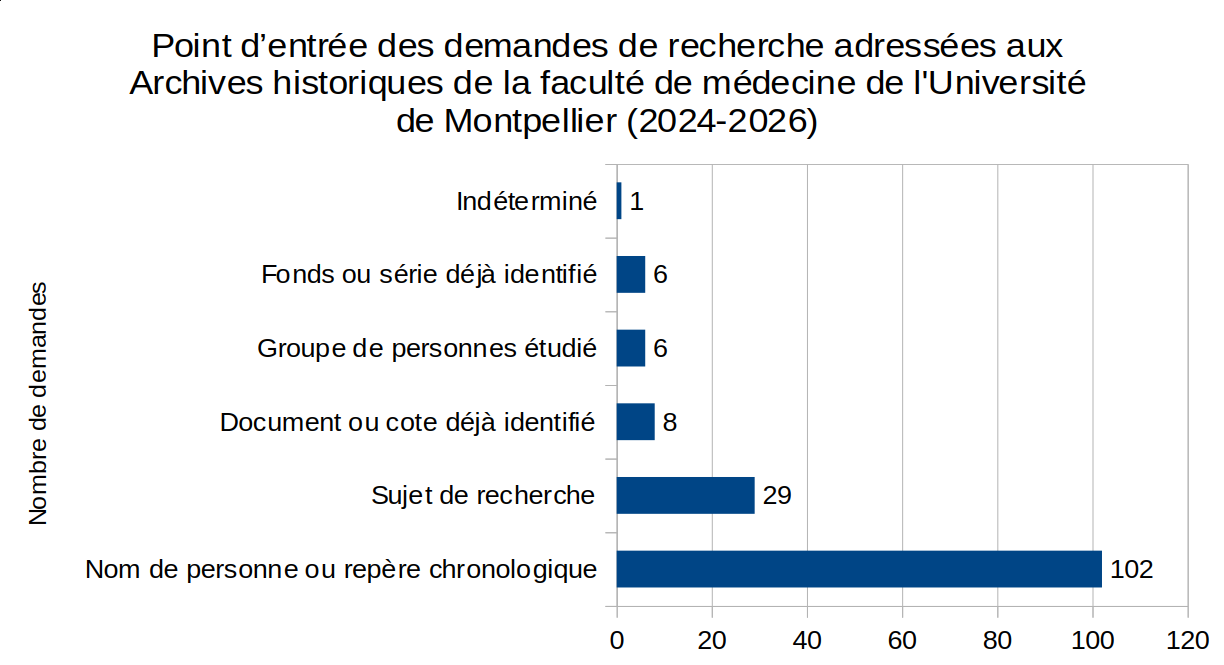
\includegraphics[width=0.88\textwidth]{images/point_entree_demandes_2024-2026.png}
	\caption[Point d'entrée des demandes de recherche, 2024--2026]
	{Point d'entrée des demandes de recherche adressées aux Archives historiques de la Faculté de médecine de l'Université de Montpellier entre 2024 et la pause estivale de la mi-juillet 2026. Graphique réalisé par Clara Martin à partir des données du suivi des demandes renseignées par la Mission Archives historiques.}
	\label{fig:point-entree-demandes}
\end{figure}

Ces chiffres renseignent moins sur la précision des demandes que sur la connaissance de l'organisation documentaire. Une recherche peut être clairement définie --- retrouver le parcours d'une personne à une date donnée, par exemple --- sans que son auteur sache dans quelle série ou sous quelle cote se trouve l'information. Le phénomène est particulièrement net pour la scolarité et les parcours universitaires : 103 demandes relèvent de cet objet, dont 86 prennent pour point d'entrée un nom de personne ou un repère chronologique. L'identification des registres, dossiers d'étudiants ou autres archives administratives pertinents repose alors sur le service.

Les consultations sur place présentent un profil différent. Comme pour les demandes par correspondance, chaque séance a été rattachée à un objet principal, déterminé d'après l'information recherchée plutôt que d'après les fonds mobilisés. Sur 76 séances, 25 concernent la scolarité et les parcours universitaires, soit 32,9\,\% ; 17 les enseignements, les pratiques et les savoirs médicaux ; 14 le patrimoine, les bâtiments et les collections ; 10 la vie et la carrière d'une personne ; et huit le gouvernement et l'histoire institutionnelle. Une séance relève de la catégorie \enquote{autre} et une demeure indéterminée. Plusieurs ensembles pouvant être consultés au cours d'une même séance, ces 76 consultations représentent 110 occurrences de fonds.

\begin{figure}[htbp]
	\centering
	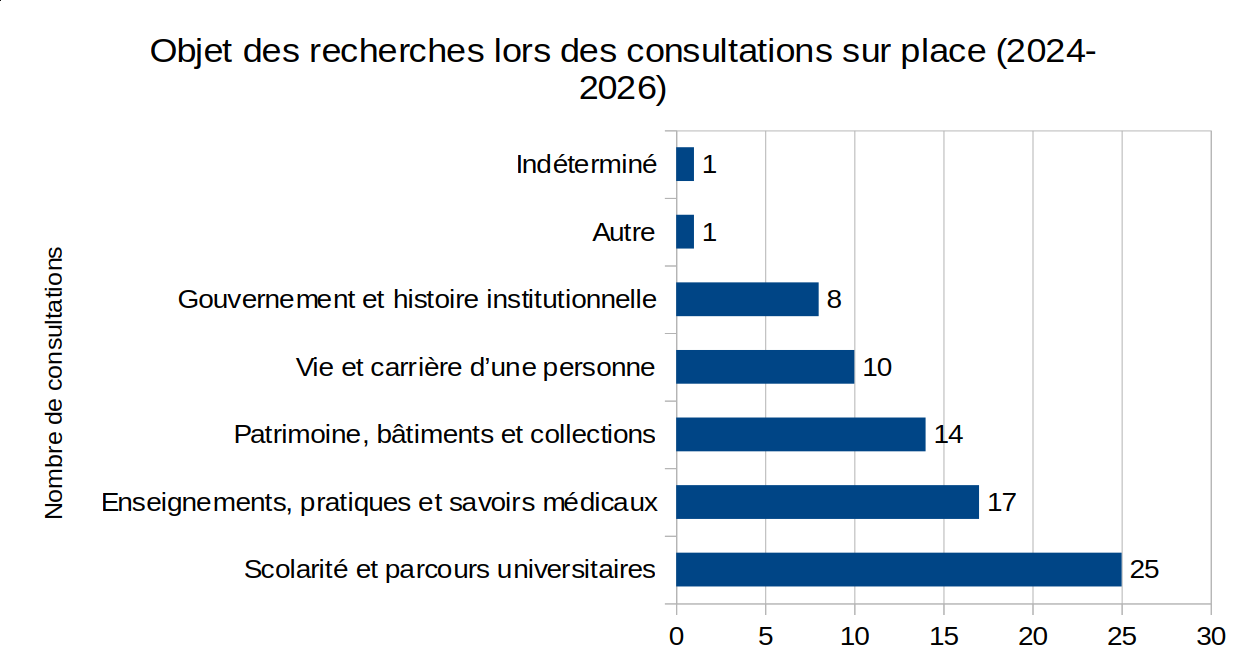
\includegraphics[width=0.88\textwidth]{images/objet_recherches_consultations_2024-2026.png}
	\caption[Objet des recherches lors des consultations sur place, 2024--2026]
	{Objet des recherches lors des consultations sur place entre 2024 et la pause estivale de la mi-juillet 2026. Graphique réalisé par Clara Martin à partir des données du suivi des consultations renseignées par la Mission Archives historiques.}
	\label{fig:objet-consultations}
\end{figure}

Cette différence tient en partie à la nature des recherches. Une demande familiale ou généalogique portant sur un parcours universitaire peut souvent être satisfaite par la vérification d'une mention et l'envoi de quelques reproductions ; une recherche universitaire ou érudite nécessite plus fréquemment la consultation suivie et croisée de plusieurs documents. La mise en ligne ne répond donc pas de la même manière à tous les usages : l'amélioration du \gls{signalement} peut bénéficier à l'ensemble des chercheurs, tandis que la numérisation présente un intérêt particulier pour les corpus faisant l'objet de demandes nominatives répétées.

Un premier besoin fonctionnel apparaît ainsi : permettre aux usagers de passer plus facilement de leur objet de recherche aux ensembles documentaires susceptibles d'y répondre, alors que cette identification repose encore largement sur la connaissance des fonds détenue par le personnel.

\paragraph{Une médiation documentaire qui représente une charge de travail mesurable}

Les 76 séances recensées entre 2024 et la pause estivale de la mi-juillet 2026 représentent 9\,955 minutes de consultation sur place, soit 165~h~55, auxquelles s'ajoutent 1\,150 minutes de préparation renseignées, soit 19~h~10. Le total documenté atteint ainsi 11\,105 minutes, soit un peu plus de 185 heures.

\begin{table}[htbp]
	\centering
	\small
	\caption{Temps mobilisé par les consultations sur place}
	\label{tab:temps-consultations}
	\begin{tabular}{lrrrr}
		\toprule
		\textbf{Année} &
		\textbf{Séances} &
		\textbf{Consultation (min)} &
		\textbf{Préparation (min)} &
		\textbf{Total (min)} \\
		\midrule
		2024 & 35 & 4\,575 & 55  & 4\,630 \\
		2025 & 23 & 3\,025 & 755 & 3\,780 \\
		2026 & 18 & 2\,355 & 340 & 2\,695 \\
		\midrule
		\textbf{Total} & \textbf{76} & \textbf{9\,955} & \textbf{1\,150} & \textbf{11\,105} \\
		\bottomrule
	\end{tabular}
	
	\vspace{0.3em}
	\begin{minipage}{0.93\textwidth}
		\footnotesize
		\emph{Source :} tableau élaboré par Clara Martin à partir des données du suivi des consultations renseignées par la Mission Archives historiques. Le temps de préparation n'était pas systématiquement indiqué, notamment en 2024 ; les valeurs présentées constituent donc un minimum. Les données de 2026 sont arrêtées à la pause estivale de la mi-juillet.
	\end{minipage}
\end{table}

Les 152 demandes traitées par correspondance représentent en outre 4\,485 minutes de travail renseigné, soit 74~h~45. Ce relevé demeure lui aussi partiel : le temps consacré à cinq demandes n'a pas été renseigné et les données de 2026 s'arrêtent à la mi-juillet. Ces chiffres ne permettent pas d'estimer directement le temps que ferait économiser une amélioration de l'accès en ligne, mais montrent qu'une part mesurable de l'activité est consacrée à identifier les sources, à préparer leur communication et à répondre individuellement aux demandes.

Pour 2025 et la période étudiée de 2026, 197 numérisations sont explicitement comptabilisées dans 32 envois dont le nombre d'images est renseigné ; 193 d'entre elles répondent à des demandes externes. La reproduction constitue donc déjà un mode courant de communication à distance. Pour certaines recherches nominatives, notamment relatives à la scolarité, la réponse consiste à repérer une mention dans un registre puis à en transmettre la reproduction. La mise en ligne des registres les plus sollicités pourrait éviter une partie de ces opérations répétées ; le même raisonnement vaut, dans une moindre mesure, pour certains registres anciens régulièrement demandés.

La publication des instruments de recherche répond à un besoin différent. Elle ne supprimera ni les demandes ni la médiation archivistique, mais elle peut permettre aux chercheurs d'effectuer eux-mêmes un premier repérage et d'adresser des demandes mieux documentées. Une meilleure visibilité peut parallèlement susciter de nouvelles recherches et consultations : l'objectif n'est donc pas simplement de réduire la charge de travail, mais d'éviter que le service assume systématiquement des opérations élémentaires pouvant être effectuées par l'usager, afin de concentrer sa médiation sur les recherches nécessitant réellement sa connaissance des fonds.

Deux besoins complémentaires se dégagent ainsi : signaler les fonds et les unités documentaires pertinents, puis donner sélectivement accès aux reproductions des corpus les plus sollicités.

\chapter{Structuration, publication et signalement des descriptions archivistiques}
\chapitrecourt{Signalement des descriptions archivistiques}

\section{Le mini-site institutionnel comme espace de médiation et de valorisation}

La création d'un mini-site institutionnel répond à un besoin distinct de ceux auxquels doivent satisfaire les outils de description et de diffusion examinés dans la suite de ce chapitre. Sans constituer une nouvelle base documentaire ni accueillir la production des instruments de recherche, il doit organiser l'accès aux fonds, aux instruments publiés, aux informations pratiques, aux contenus de valorisation et, le cas échéant, aux reproductions diffusées dans d'autres environnements.

Cette fonction a été éprouvée pendant le stage par un premier prototype développé localement en HTML, CSS et JavaScript, puis par sa transposition dans un environnement WordPress de préproduction de l'Université\footnote{Le contenu du prototype, ses choix éditoriaux, ses limites, son code source et sa version consultable sont présentés en annexe~\ref{annexe:prototype-mini-site}.}. Le premier permettait d'expérimenter librement l'organisation des contenus et les parcours de navigation ; le second confrontait ces choix aux conditions institutionnelles de publication. Le prototypage visait ainsi moins à préfigurer techniquement le site définitif qu'à déterminer les fonctions susceptibles d'être confiées à cette interface éditoriale.

\subsection{Expérimenter plusieurs parcours d'accès aux fonds}

Le prototype distingue quatre entrées principales --- l'accueil, les fonds et instruments de recherche, les expositions et la consultation --- auxquelles s'ajoute une restitution numérique du \enquote{musée des archives}. Elles correspondent à des intentions différentes : découvrir le service et ses fonds, identifier des documents, préparer leur consultation ou parcourir les archives à partir d'un récit ou d'une sélection patrimoniale.

Une interface consacrée à des collections ne peut présupposer que ses utilisateurs connaissent déjà la ressource recherchée. Si la requête répond efficacement à un besoin défini, elle rend moins perceptibles l'étendue et la diversité d'un ensemble documentaire ; des interfaces donnant davantage à voir les collections favorisent au contraire l'exploration, la découverte et le passage d'une vue générale à des ressources particulières\footcite{Whitelaw2015GenerousInterfaces}. Cette complémentarité correspond à la diversité des usages envisageables pour les archives historiques, depuis la recherche d'une cote précise jusqu'à une première découverte des fonds.

La rubrique documentaire donne donc une vue d'ensemble des fonds avant de conduire, lorsqu'ils existent, vers leurs instruments. Pour chaque instrument disponible sont indiqués sa cote, son intitulé, une courte description et un lien vers le PDF ou la ressource diffusée dans un autre environnement. Seuls les trois instruments déjà publiés en ligne --- les répertoires 1MED, 2MED et 1FiMED --- ont été intégrés ; les autres ensembles restent signalés sans donner accès à leurs instruments internes ou non publiés. Lors de la transposition du prototype local dans WordPress, la page qui réunissait initialement les fonds publics modernes et contemporains et les fonds privés a ainsi été répartie entre trois ensembles --- fonds ancien, fonds modernes et contemporains publics, et fonds privés --- afin d'en rendre l'organisation plus lisible.

Cette organisation privilégie un espace spécifiquement consacré aux archives plutôt que la dispersion de pages dans les rubriques thématiques du site institutionnel. Si cette dernière solution rapproche les activités passées et présentes, elle tend à privilégier les ensembles qui s'y prêtent le mieux ; un espace dédié permet de représenter plus largement les fonds communicables\footcite[pp.~94--95]{FerradouFine2011}.

Les plans de classement, encore en cours d'élaboration au moment du mémoire, n'ont pas été intégrés. À terme, une arborescence pourrait rendre visibles tous les ensembles conservés, y compris ceux dépourvus d'instrument publié, tandis que des notices synthétiques préciseraient leur contenu général, leurs dates extrêmes et leur état de traitement. Lorsqu'un instrument est disponible, un lien conduirait à sa présentation détaillée. La rubrique remplirait ainsi une fonction d'état général des fonds tout en distinguant leur existence, leur traitement archivistique et la publication de leurs instruments.

\subsection{Accompagner l'utilisateur vers les instruments de recherche}

Rendre les fonds visibles ne suffit pas à rendre leur organisation intelligible. Les instruments de recherche préservent la provenance, la hiérarchie et le contexte documentaire selon des principes et un vocabulaire qui ne correspondent pas nécessairement aux catégories à partir desquelles un utilisateur formule sa recherche. La description à plusieurs niveaux et des termes tels que \enquote{instrument de recherche}, \enquote{état des fonds} ou \enquote{cadre de classement} peuvent ainsi constituer des obstacles\footcite[pp.~25--26]{Homer2021}.

La diffusion sur le web accentue cette difficulté en éloignant l'instrument du contexte dans lequel sa consultation pouvait être accompagnée par un archiviste. La conformité aux standards descriptifs reste nécessaire, mais ne garantit pas à elle seule l'usage d'un instrument en ligne : terminologie, représentation de la hiérarchie, fonctions de recherche et présentation de l'information interviennent également\footcite[pp.~24--27]{AlfierFeliciati2017}. Des tests menés auprès d'utilisateurs montrent notamment les difficultés provoquées par des intitulés ambigus, des relations de navigation insuffisamment explicites, le jargon professionnel ou des hiérarchies dans lesquelles il devient difficile de se situer\footcite[pp.~30--35]{Walton2017FindingAids}.

Le mini-site ajoute donc un niveau d'explication sans modifier la structure scientifique des instruments. Une rubrique d'aide a été conçue pour expliquer l'organisation en fonds, le rôle de la cote ainsi que la localisation et la lecture des inventaires. Des formulations comme \enquote{fonds et collections} ou \enquote{recherche dans les inventaires} peuvent être plus accessibles que \enquote{cadre de classement}, tandis que les \enquote{archives numérisées} doivent être distinguées des autres ressources proposées en ligne\footcite[p.~28]{Homer2021}. Le vocabulaire archivistique n'est pas supprimé, mais introduit au moment où il devient nécessaire au parcours.

La mise en ligne d'un instrument ne garantit d'ailleurs pas son utilisation. Dans une enquête menée auprès des internautes des Archives départementales du Var, 95\,\% des répondants déclaraient consulter les documents numérisés, contre seulement 20\,\% les instruments de recherche, dont l'offre en ligne restait alors partielle\footcite[p.~154]{BugatDroguetJegouzo2007}. Sans transposer ces proportions au cas montpelliérain, cet écart distingue nettement disponibilité documentaire et appropriation des outils de repérage. Les Archives départementales de la Vendée proposaient ainsi un accès thématique destiné aux non-initiés parallèlement à un état des fonds davantage conçu pour les chercheurs familiers de l'organisation archivistique, complétés par des fiches méthodologiques guidant les recherches à partir d'objets concrets\footcite[p.~141]{Roy2012}.

La page consacrée à la consultation prolonge cette médiation jusqu'à l'accès physique aux documents. Elle rassemble les conditions d'accès, les coordonnées de la Mission et les informations utiles à une demande --- sujet de recherche, fonds ou cote éventuellement repérés, dates ou personnes concernées --- et explique comment identifier une cote et parcourir un inventaire. Liens internes, renvois vers les instruments et modalités de contact clairement indiquées doivent assurer la circulation entre ces différents niveaux d'information\footcite[p.~96]{FerradouFine2011}. Le mini-site prépare ainsi la recherche sans prétendre remplacer l'accompagnement archivistique lorsqu'il reste nécessaire.

Les documents rencontrés au cours de ces parcours doivent enfin demeurer reliés aux descriptions qui les contextualisent. Dans le cas des Arts Décoratifs, numérisation, documentation et indexation forment une même chaîne, tandis que thésaurus et mots-clés constituent des \enquote{passerelles} entre professionnels, amateurs et chercheurs\footcite[pp.~222--223]{Collin2017}. Pour les archives historiques, cette articulation conduit à permettre le passage entre document, fonds et instrument plutôt qu'à isoler les ressources de médiation de leur contexte archivistique.

\subsection{Reconstituer le \enquote{musée des archives} : faire de l'histoire de la valorisation un objet de médiation}

Le prototype a également permis d'expérimenter une forme de valorisation qui ne préexistait pas sous forme numérique. La rubrique consacrée aux expositions donne accès à l'exposition virtuelle \enquote{14--18, Médecine au champ d'honneur}\footcite{UMExpositionMedecine1418} ainsi qu'à la présentation et au livret numériques de l'exposition \enquote{Les Bâtisseurs de la Faculté de médecine du XX\textsuperscript{e} siècle}\footcite{BatisseursFaculte2021}\footcite{BatisseursFaculte2021Livret}. À ces ressources existantes s'ajoute une proposition conçue pendant le stage : la reconstitution numérique du \enquote{musée des archives} constitué par Joseph Calmette au début du XX\textsuperscript{e} siècle.

Après l'achèvement du classement du fonds ancien en 1908, Calmette avait disposé dans une vitrine du Musée Atger une sélection de pièces remarquables, dont il publia la liste dans le second tome du \emph{Cartulaire de l'Université de Montpellier}. Ces spécimens devaient donner un aperçu de la variété et de l'intérêt des archives et éveiller la curiosité des visiteurs pour l'histoire de la Faculté\footcite[p.~XVI--XXI, vues~35 à 40 de la version numérisée]{CalmetteCartulaire1912}. Aujourd'hui disparue, cette vitrine appartient elle-même à l'histoire de la patrimonialisation du fonds : le reclassement des archives anciennes s'accompagnait de leur exposition comme objets historiques.

La reconstitution reprend les vingt-deux pièces de cette sélection, chacune associée à sa cote, sa date, une courte présentation et une reproduction ; l'interface permet de parcourir l'ensemble ou d'accéder directement à une pièce et d'en agrandir l'image\footnote{Les reproductions ont été réalisées par Clara Martin au cours du stage. Certains documents, notamment des parchemins de la série B, ont été numérisés dans leur état matériel actuel et apparaissent donc encore pliés. Leur mise à plat et leur restauration doivent être effectuées ultérieurement par les ateliers du \gls{scdi}.}. Il ne s'agit donc ni de constituer une nouvelle sélection de \enquote{trésors} ni d'en faire un instrument de recherche autonome, mais de prendre pour objet un choix historique déjà constitué.

Le passage de la vitrine au dispositif numérique en transforme cependant les modalités d'exploration. Les pièces deviennent individuellement accessibles, tandis que leur cote et leur contextualisation permettent de revenir de l'objet remarquable vers l'ensemble archivistique auquel il appartient. Cette circulation entre vue d'ensemble, exploration et détail correspond aux possibilités d'interfaces patrimoniales qui ne réduisent pas l'accès aux collections à la formulation préalable d'une requête\footcite{Whitelaw2015GenerousInterfaces}. La reconstitution conserve ainsi le principe de la sélection de Calmette sans chercher à reproduire matériellement sa vitrine.

Elle rend simultanément accessibles les documents choisis et le geste qui les avait réunis. La liste publiée par Calmette devient la source permettant de restituer une manière historiquement située de présenter les archives de la Faculté. L'histoire du traitement et de la valorisation du fonds, étudiée dans la première partie, fournit ainsi elle-même la matière d'une expérimentation numérique contemporaine.

Pour les futurs contenus éditoriaux, le choix des pièces répondrait à d'autres critères. Les fonds retenus pour une valorisation institutionnelle doivent notamment être communicables, représentatifs de l'activité de l'établissement, liés aux thématiques traitées, suffisamment décrits et dotés d'un potentiel iconographique ; les documents les plus attractifs peuvent alors conduire vers des ensembles visuellement plus sobres mais plus riches sur le plan scientifique\footcite[pp.~92--94]{FerradouFine2011}. La valorisation repose ainsi sur une \enquote{mise en perspective et en contexte porteuse de sens}, tandis que le choix de l'outil doit découler du discours et des documents à présenter\footcite[pp.~363--366]{GueitMontchal2019}. La reconstitution du \enquote{musée des archives} en fournit ici une application : sa forme découle de l'objet historique qu'elle cherche à restituer.

\begin{figure}[htbp]
	\centering
	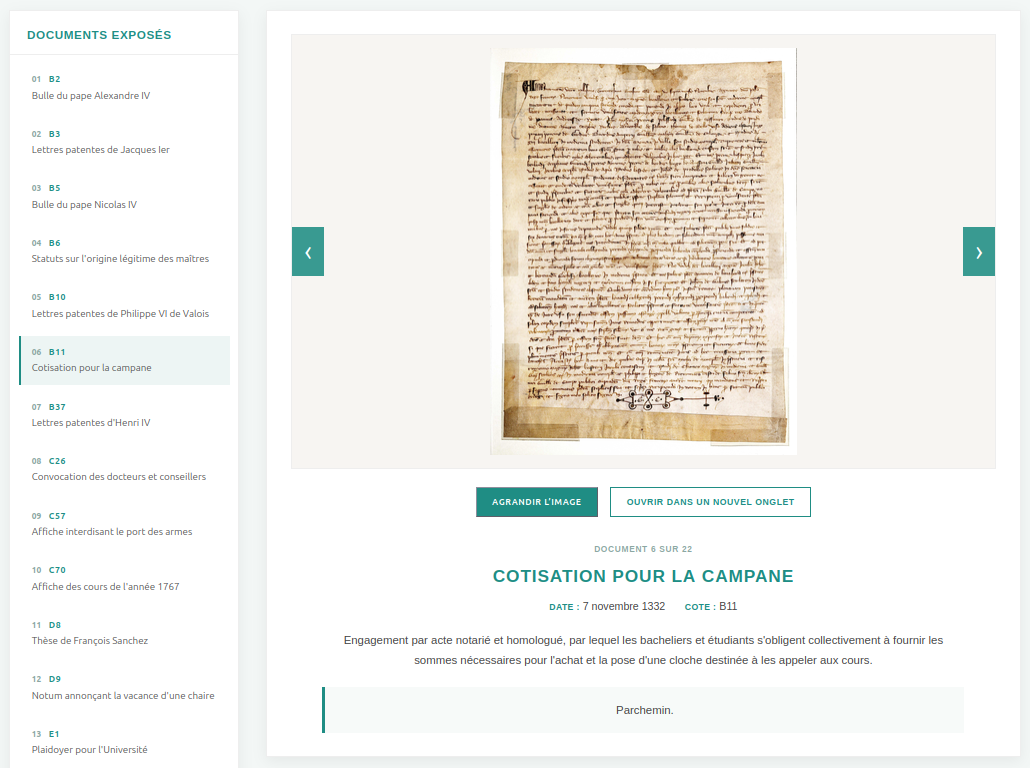
\includegraphics[width=\textwidth]{images/musee_des_archives.png}
	\caption{Prototype de restitution numérique du \enquote{musée des archives} de Joseph Calmette : navigation dans la sélection et contextualisation d'une pièce}
	\label{fig:prototype-musee-archives}
\end{figure}

\subsection{Inscrire la médiation dans l'environnement institutionnel}

La transposition du prototype dans l'environnement de préproduction de l'Université permettait enfin d'éprouver sa viabilité institutionnelle. Le site principal et plusieurs mini-sites de l'Université de Montpellier reposent sur WordPress, un \gls{cms} dont le cadre graphique, fonctionnel et éditorial impose davantage de contraintes que le prototype local.

Cette intégration évite de faire dépendre durablement la diffusion des Archives historiques d'un site autonome développé pendant le stage. L'Université assure l'hébergement, la maintenance, la sécurité et les mises à jour techniques, tandis que la Mission conserve la gestion scientifique et éditoriale de ses contenus. Cette répartition rejoint un modèle de publication dans lequel les détenteurs de l'information assurent son édition initiale au sein d'un dispositif commun de validation et de publication, plutôt qu'un fonctionnement centralisé autour d'un webmestre multipliant transmissions et rééditions\footcite[pp.~122--124]{Reymond2008Webometrie}. La Mission conserve ainsi la maîtrise de ses contenus archivistiques, tandis que la \gls{dsin} encadre leur publication technique.

Cette articulation suppose une coordination entre compétences archivistiques, éditoriales et techniques. À l'agence de l'eau Adour-Garonne, l'intégration des archives au site institutionnel avait ainsi associé le service des archives, les responsables éditoriaux et techniques et des usagers internes pour déterminer la place des pages dans l'arborescence, leur articulation avec la ligne éditoriale et leur adaptation à la charte graphique\footcite[pp.~92--96]{FerradouFine2011}. Le passage du prototype local à WordPress confronte de même les besoins définis par la Mission aux règles éditoriales de l'Université et aux possibilités techniques de la \gls{dsin}.

Cette inscription donne parallèlement aux archives une place identifiable dans la communication générale de l'établissement : elle permet de toucher ses publics, de moderniser leur image auprès du personnel, de légitimer leur place dans son patrimoine intellectuel et, par une meilleure identification des fonds et de leurs conditions d'accès, de contribuer à sa transparence\footcite[pp.~90--91 et 98--103]{FerradouFine2011}.

Le cadre institutionnel fixe toutefois les limites du mini-site. L'ajout de composants et les modifications techniques demeurent encadrés, tandis que l'affichage standard de WordPress ne répond pas aux besoins de consultation précise des manuscrits, parchemins, registres ou documents de grand format. Les échanges avec la \gls{dsin} et le service de la communication ont montré que des développements spécifiques, notamment l'intégration d'une visionneuse, restaient envisageables.\footnote{Les solutions permettant d'articuler descriptions archivistiques et reproductions numériques sont examinées au chapitre~\ref{chap:articulation-descriptions-reproductions}.} Le stockage et la diffusion des reproductions relèvent cependant d'autres dispositifs, de même que la production et la maintenance des instruments de recherche, qui doivent pouvoir être structurés, corrigés et actualisés sans ressaisie dans WordPress.

Une logique de \enquote{dissémination} peut précisément associer un site institutionnel consacré à l'orientation et à la médiation à des dispositifs distincts pour l'accès aux collections numérisées\footcite[p.~156]{Halais2012}. Le prototype permet ainsi de circonscrire la fonction du mini-site dans l'architecture de diffusion : rendre les fonds visibles, expliquer leur organisation, accompagner l'accès aux instruments, proposer des parcours de valorisation et orienter vers les ressources diffusées ailleurs. La production, la structuration et le \gls{signalement} des instruments relèvent dès lors d'outils spécialisés, qu'il convient maintenant d'examiner.

\section{La structuration et le signalement des instruments de recherche en EAD}
\label{sec:structuration-signalement-ead}

\subsection{L'EAD, format commun de structuration et d'échange}
\label{subsec:ead-format-echange}

\paragraph{La structure de la description archivistique}

La \gls{ead}, ou Description archivistique encodée, est un standard conçu pour représenter les instruments de recherche archivistiques sous une forme structurée. Développée à partir des années 1990 à l'initiative de la Society of American Archivists, elle répond aux besoins d'échange apparus avec l'informatisation des services d'archives et la diffusion des descriptions sur le web\footcite[pp.~84--85]{Sibille2012}.

L'\gls{ead} repose sur le \gls{xml}, syntaxe générique permettant de hiérarchiser, de contrôler, d'interroger, de transformer et d'échanger des données. Elle lui associe un vocabulaire propre à la description archivistique : l'\gls{ead} 2002 prévoit notamment des éléments pour la cote (\texttt{<unitid>}), l'intitulé (\texttt{<unittitle>}), les dates (\texttt{<unitdate>}), le producteur (\texttt{<origination>}) ou la présentation du contenu (\texttt{<scopecontent>})\footcite{EAD2002Dictionnaire}. La fonction de chaque information devient ainsi explicite et exploitable indépendamment de sa mise en page.

Les composants emboîtés restituent l'organisation d'un fonds, de ses principales subdivisions jusqu'aux dossiers ou aux pièces. Ils permettent de mettre en œuvre les quatre principes de la description à plusieurs niveaux formalisés par la norme \gls{isadg} : description du général au particulier, adaptation des informations au niveau décrit, mise en relation des niveaux et non-répétition des informations\footcite[pp.~12--13]{ISADG2000}. Les deux \glspl{referentiel} ne se confondent donc pas : \gls{isadg} définit les principes de la description, tandis que l'\gls{ead} fournit une structure informatique pour les encoder\footcite{EAD2002Dictionnaire}.

\paragraph{Un format d'échange et d'interopérabilité}

La séparation entre les données et leur restitution permet d'exploiter un même instrument dans plusieurs environnements : affichage dans une interface de consultation, transmission à un autre système, agrégation dans un catalogue collectif ou production de nouvelles restitutions. À la différence d'un fichier Word ou PDF, dont les informations restent liées à une présentation déterminée, l'\gls{ead} rend leurs composantes accessibles à des traitements automatisés\footnote{Il s'agit notamment de la validation par rapport à un schéma ou à une \gls{dtd}, de l'interrogation et de l'extraction ciblées, de l'indexation par un moteur de recherche, de la transformation au moyen de feuilles de style XSLT ou de la conversion vers d'autres formats à partir d'une même source \gls{xml}.}.

La normalisation contribue ainsi à homogénéiser et à décloisonner les descriptions produites par différentes institutions\footcite[pp.~121--122]{Motte2015}. Elle ne suffit toutefois pas à garantir leur \gls{interoperabilite} : des standards peuvent décrire des objets distincts selon des granularités différentes, de sorte que leur articulation exige une analyse des modèles et la définition de correspondances explicites\footcite{MirandaEtAl2025}.

Pour les Archives historiques de la Faculté de médecine, l'\gls{ead} fournit un cadre commun pour reprendre des instruments aujourd'hui conservés sous forme de fichiers Word, PDF ou de tableaux. Il permet surtout de dissocier les descriptions de leur interface de publication, afin de les corriger et de les réutiliser dans plusieurs dispositifs sans les ressaisir.

L'\gls{ead} 2002 demeure la version employée à la BnF et dans la très grande majorité des institutions françaises\footcite{BnFEADGeneralites}. Cette persistance coexiste avec l'évolution internationale du standard : l'\gls{ead}~4 a été officiellement lancé le 31 juillet 2026\footcite{EAD4Release2026}. Les expérimentations conduites pendant le stage ont néanmoins porté sur l'\gls{ead} 2002, qui correspond aux chaînes de traitement étudiées.

\paragraph{La préparation de la rétroconversion}

La \gls{retroconversion} ne consiste pas à remplacer mécaniquement des éléments de mise en page par des balises. Elle suppose d'identifier la fonction archivistique des informations et de reconstruire les relations parfois seulement matérialisées par des titres, des retraits ou des changements de style. Une même présentation peut recouvrir des fonctions différentes selon les instruments ; inversement, une relation hiérarchique peut être exprimée sans être explicitement désignée.

Les retours d'expérience recommandent donc d'identifier des familles d'instruments suffisamment régulières, puis de définir pour chacune un modèle cible et des règles de conversion documentées\footcite{GouletMaftei2006}\footcite{Meissner1997}. Les correspondances stables peuvent être automatisées, tandis que les ambiguïtés de structure, les variations de rédaction et les informations implicites nécessitent un contrôle archivistique.

Le chantier de dématérialisation des Archives nationales reposait ainsi sur des consignes établies pour chaque instrument et sur une chaîne distinguant numérisation, restitution du texte, encodage et saisie des cotes, avec un contrôle propre à chaque opération\footcite[pp.~199--202]{Aristide2010}. L'analyse conduite pendant le stage a suivi une logique comparable : repérage des structures récurrentes, détermination des informations normalisables, formalisation de règles de saisie et contrôle de la restitution des cotes et des niveaux. Ce travail préparatoire a permis d'évaluer plusieurs chaînes de production de fichiers en \gls{ead} adaptées aux moyens du service.

\subsection{L'identification institutionnelle, préalable au signalement}
\label{subsec:identification-institutionnelle}

La circulation des descriptions suppose d'identifier de manière univoque l'institution qui en assume la responsabilité. La \gls{isdiah} fait ainsi de l'identifiant un élément obligatoire de la description des institutions conservant des archives et prévoit l'enregistrement d'un code unique conforme aux normes nationales et internationales applicables\footcite[pp.~13 et 16]{ISDIAH2008}. La norme \gls{isadg} l'intègre à la référence des unités de description, composée notamment du code du pays, du code du service d'archives et de la cote locale\footcite{ISADG2000}.

En France, l'identifiant unique des services d'archives est attribué par le \gls{siaf}, seul habilité à le délivrer\footcite[p.~4]{SIAFEnquete2025}. Il intervient également dans la construction de l'identifiant unique des entrées\footcite{SchemaRegistreEntrees}.

La position institutionnelle particulière de la Mission Archives historiques ne permet pas de déterminer directement le code sous lequel signaler ses fonds.\footnote{Cette position institutionnelle est exposée au chapitre~\ref{chap:cadre-juridique-derogation}.} La consultation du \gls{siaf} doit donc établir si les descriptions peuvent être rattachées à un identifiant existant ou si un identifiant propre doit être attribué. Cette clarification n'empêche pas leur structuration en \gls{ead}, mais conditionne leur versement effectif dans FranceArchives.

\subsection{SimplEAD : une chaîne légère de rétroconversion vers FranceArchives}
\label{subsec:simplead-francearchives}

\paragraph{Le signalement dans FranceArchives}

Mis en ligne en 2017 par le Service interministériel des Archives de France (\gls{siaf}), FranceArchives agrège et rend interrogeables dans un moteur fédéré les instruments de recherche d'institutions et de services publics ou privés, produits dans des environnements techniques hétérogènes\footcite[pp.~34--35]{Restif2021}. Le portail offre ainsi un point d'accès commun à leurs descriptions sans se substituer aux institutions de conservation ni à leurs propres interfaces. Il n'héberge pas les images numérisées, mais peut renvoyer vers les reproductions consultables sur les sites sources\footcite{FranceArchivesContenu}\footcite{FranceArchivesRejoindre2026}. Pour les Archives historiques, ce référencement national compléterait donc la diffusion assurée par l'Université.

En 2021, environ 80\,\% des instruments intégrés étaient encodés en \gls{ead} ; des fichiers PDF ou CSV accompagnés de \glspl{metadonnees} en Dublin Core pouvaient également être reçus\footcite[p.~36]{Restif2021}. L'alimentation s'effectue par transmission de fichiers ou, lorsque le contributeur dispose de l'infrastructure nécessaire, par récupération automatisée de ses données\footcite{FranceArchivesRejoindre2026}. SimplEAD répond au cas des services qui ne produisent pas directement de fichiers en \gls{ead}.

\paragraph{L'organisation du modèle d'import}

SimplEAD convertit en \gls{xml}-\gls{ead} 2002 un instrument préparé dans un modèle tabulaire disponible aux formats Excel (\texttt{.xlsx}) et OpenDocument (\texttt{.ods})\footcite{FranceArchivesSimplEAD}. Les données sont saisies localement, puis le fichier est chargé dans le convertisseur, qui génère le document \gls{ead} sans exiger la rédaction directe du code \gls{xml} ni le déploiement d'un système d'information archivistique.

La chaîne a été expérimentée sur quatre instruments présentant des structures différentes : les archives relatives aux legs Bouisson-Bertrand et Jaumes (\texttt{LEG}), celles de la maïeutique (\texttt{MAIE}), le fonds d'affiches de la Faculté (\texttt{1 Fi/MED}) et le sous-fonds consacré à la transfusion sanguine d'Émile Jeanbrau (\texttt{1EJ}). Le périmètre de FranceArchives incluant les descriptions produites par des institutions privées, la nature juridique de certains de ces fonds ne constitue pas un obstacle à leur \gls{signalement}\footcite[p.~35]{Restif2021}.

Le modèle d'import fourni par SimplEAD comporte trois feuilles, dont les fonctions et les correspondances avec l'\gls{ead} sont distinctes\footcite{FranceArchivesSimplEADDocumentation}.

\begin{table}[htbp]
	\centering
	\scriptsize
	\setlength{\tabcolsep}{4pt}
	\renewcommand{\arraystretch}{1.15}
	\caption{Structure du modèle d'import SimplEAD utilisé pendant l'expérimentation}
	\label{tab:structure-simplead}
	
	\begin{tabularx}{\textwidth}{
			>{\raggedright\arraybackslash}p{2.7cm}
			>{\raggedright\arraybackslash}p{3.1cm}
			>{\raggedright\arraybackslash}X
		}
		\toprule
		\textbf{Feuille} &
		\textbf{Fonction} &
		\textbf{Champs} \\
		\midrule
		
		\texttt{intitulé\_inventaire} &
		Identification et responsabilité de l'instrument ; identification du producteur &
		Identifiant de l'inventaire ; titre ; sous-titre ; responsable de la conservation ; adresse ; date de publication ; auteur ; producteur ; type de producteur. \\
		
		\addlinespace
		
		\texttt{description\_du\_fonds} &
		Description de haut niveau correspondant principalement à \texttt{archdesc} &
		Titre ; dates de début et de fin ; description physique ; cote ; description du contenu ; indexation par lieu, personne, institution et matière ; conditions d'accès ; niveau de description de l'inventaire ; langue ; conditions d'utilisation et de reproduction ; modalité d'entrée. \\
		
		\addlinespace
		
		\texttt{description\_cotes} &
		Description hiérarchisée des unités documentaires au moyen de composants \texttt{<c>} &
		Niveau ; titre ; cote ; dates de début et de fin ; description physique ; description du contenu ; indexation par lieu, personne, institution et matière ; conditions d'accès ; profondeur de la description archivistique. \\
		
		\bottomrule
	\end{tabularx}
	
	\vspace{0.3em}
	
	\begin{minipage}{0.95\textwidth}
		\footnotesize
		\emph{Source :} modèle d'import SimplEAD utilisé dans le cadre du stage et documentation du Service interministériel des Archives de France.
	\end{minipage}
\end{table}

La première feuille ne correspond pas intégralement à un seul bloc de l'\gls{ead}. Les informations éditoriales alimentent notamment \texttt{eadheader}, tandis que les champs \enquote{Producteur} et \enquote{Type de producteur} sont convertis en \texttt{origination} et en \texttt{persname} ou \texttt{corpname}. L'identifiant de l'instrument doit être unique, pérenne et préfixé par le code du service contributeur.\footnote{La détermination de ce code est examinée à la sous-section~\ref{subsec:identification-institutionnelle}.} Le sous-titre n'étant exploité ni par FranceArchives ni par le portail européen des archives, il ne doit pas contenir une information indispensable au repérage de l'instrument\footcite{FranceArchivesSimplEADDocumentation}.

Plusieurs valeurs d'indexation de même nature sont séparées par une arobase, tandis que des listes déroulantes contrôlent certains champs afin de limiter les variantes de saisie\footcite{FranceArchivesSimplEAD}\footcite{FranceArchivesSimplEADDocumentation}. La qualité du \gls{signalement} dépend néanmoins de la normalisation des points d'accès. La documentation recommande l'emploi des formes d'autorité proposées par FranceArchives, l'hétérogénéité de la description et de l'indexation constituant l'une des principales difficultés d'exploitation des données agrégées\footcite{FranceArchivesSimplEADDocumentation}\footcite[p.~40]{Restif2021}.

\paragraph{La restitution de la hiérarchie}

SimplEAD distingue la position d'une unité dans l'arborescence de son niveau archivistique. La colonne \enquote{Niveau} attribue à chaque ligne un rang compris entre 1 et 5 et commande l'emboîtement des composants. La colonne \enquote{Profondeur de la description archivistique} qualifie l'unité décrite et alimente l'attribut \texttt{@level} de l'élément \texttt{<c>}\footcite{FranceArchivesSimplEADDocumentation}. Sa liste contrôlée comprend notamment \enquote{groupe de documents}, \enquote{sous-groupe de documents}, \enquote{série organique}, \enquote{sous-série organique}, \enquote{dossier}, \enquote{pièce} et \enquote{autre niveau de description}.

Ces informations sont indépendantes : une unité placée au cinquième rang peut décrire un dossier, tandis qu'un dossier peut apparaître au deuxième rang dans une arborescence moins développée. De même, une rubrique ne doit être qualifiée de \enquote{série organique} que si elle correspond à un ensemble constitué par l'activité du producteur ; lorsqu'elle résulte du classement, \enquote{groupe de documents} ou \enquote{sous-groupe de documents} constitue une qualification plus appropriée.

L'instrument \texttt{MAIE} a permis de tester les cinq rangs disponibles. La branche consacrée aux inscriptions enchaîne \enquote{Gestion de l'enseignement} au niveau 1, \enquote{Organisation des études} au niveau 2, \enquote{Inscriptions} au niveau 3, \enquote{Fiches d'inscription} au niveau 4, puis les dossiers \texttt{MAIE55} et \texttt{MAIE56} au niveau 5. Les quatre premiers composants organisent intellectuellement les dossiers décrits au dernier niveau.

Le rattachement dépend de l'ordre des lignes. Une unité de niveau 5 relève du dernier niveau 4 qui la précède ; plusieurs lignes successives de niveau 5 constituent des unités sœurs. Le retour de 5 à 3 ferme les niveaux 5 et 4 avant d'ouvrir une nouvelle branche sous le dernier niveau 2 rencontré. De même, le passage de 4 à 1 clôt toute la branche précédente avant d'ouvrir un nouveau composant de premier niveau. Une remontée peut donc franchir plusieurs rangs sans ambiguïté ; en revanche, le passage de 3 à 5 laisserait l'unité de niveau 5 dépourvue de parent au niveau 4.

Le fichier généré doit enfin être contrôlé afin de vérifier que cette succession a été correctement traduite par l'emboîtement des composants \texttt{<c>}.

\paragraph{Une chaîne de publication, non un outil de gestion}

Les essais ont permis de générer les fichiers \gls{xml}-\gls{ead}, mais leur versement dans FranceArchives demeure subordonné à l'identification des Archives historiques comme service contributeur\footnote{Les modalités de cette identification sont exposées à la sous-section~\ref{subsec:identification-institutionnelle} et ses conséquences sur le choix de la chaîne sont reprises dans la conclusion du chapitre.}.

SimplEAD offre une solution proportionnée pour convertir et signaler des instruments stabilisés sans déployer immédiatement un système d'information archivistique. Il ne constitue toutefois ni un environnement de production partagée ni un outil de maintenance : les fichiers sources restent conservés localement et toute correction impose une nouvelle conversion, puis une nouvelle transmission.

Une alimentation automatisée repose sur une autre architecture. Le protocole \gls{oaipmh} permet à un fournisseur de données d'exposer sur le web des \glspl{metadonnees} structurées en \gls{xml}, qu'un fournisseur de services récupère au moyen de requêtes \gls{http}\footcite{OAIPMH2002}. FranceArchives peut ainsi actualiser les descriptions depuis le système du contributeur sans recevoir un nouveau fichier après chaque modification\footcite{FranceArchivesRejoindre2026}.

SimplEAD répond donc à la rétroconversion ponctuelle et au \gls{signalement} national d'instruments stabilisés. Leur gestion continue appelle en revanche un environnement partagé, dont Calames fournit un autre modèle.

\subsection{Calames : un environnement de production, de maintenance et de diffusion de l'EAD}
\label{subsec:calames}

Calames, Catalogue en ligne des archives et des manuscrits de l'enseignement supérieur, permet de produire et de maintenir directement les instruments en \gls{ead}, plutôt que de les préparer dans un format intermédiaire avant conversion.

\paragraph{Un catalogue collectif fondé sur la production directe en EAD}

Développé et administré par l'\Gls{abes}, Calames est un catalogue collectif consacré aux archives et manuscrits conservés dans les établissements français de l'enseignement supérieur et de la recherche\footcite{ABESCatalogueCalames}. Il est notamment issu de la \gls{retroconversion} du \textit{Catalogue général des manuscrits des bibliothèques publiques de France} (CGM), vaste entreprise de recensement et de description des manuscrits conservés dans les bibliothèques françaises, publiée en volumes à partir du XIX\textsuperscript{e} siècle. Calames a permis de reprendre ces descriptions dans un environnement où les établissements peuvent les corriger, les enrichir et les diffuser\footcite{Nicolas2007}. Il associe ainsi un catalogue public à une application professionnelle de production et de maintenance des instruments de recherche\footcite{Nicolas2008CalamesCatalogage}. Cette triple fonction d'outil d'encodage en \gls{ead}, d'interface publique et de réseau de production était déjà mise en évidence dans le bilan prospectif réalisé par l'\Gls{abes} en 2014\footcite{ABESCalamesBilan2014}.

La production s'effectue dans Calames Pro, qui repose sur XMetaL, un éditeur de documents \gls{xml} adapté par l'\Gls{abes} aux besoins du catalogage en \gls{ead}. Son interface masque une grande partie de la syntaxe \gls{xml} tout en laissant visible la structure hiérarchique : le catalogueur intervient sur les éléments de l'instrument sans saisir directement les balises\footcite{Nicolas2008CalamesCatalogage}. L'outil permet de créer et de modifier les différents niveaux de description, d'organiser les fichiers qui composent l'instrument et d'en contrôler la publication.

Contrairement à SimplEAD, où les données sont saisies dans un tableur avant leur conversion, l'instrument est directement créé et maintenu sous une forme structurée. Une correction ou un enrichissement peut ainsi être apporté sans nouvelle \gls{retroconversion}. Un fonds peut également recevoir une description synthétique, puis être détaillé à mesure de l'avancement du classement. Calames constitue donc à la fois un environnement de catalogage, une interface de diffusion et un réseau d'expertise\footcite{LatourCalames2021}.

\paragraph{La normalisation, l'indexation et les autorités}

La production dans Calames implique une normalisation et une indexation des données. La première applique des règles communes de description afin d'assurer l'homogénéité des instruments produits par les établissements du réseau ; la seconde associe aux unités décrites des points d'accès, notamment des noms de personnes, de collectivités, de lieux ou des sujets, afin de permettre leur recherche au-delà de la seule arborescence\footcite{ABESCatalogageCalames}.

Pour les personnes et les collectivités, Calames s'articule avec IdRef (\textit{Identifiants et Référentiels}), le \gls{referentiel} d'autorités de l'\Gls{abes}. Calames Pro permet ainsi d'associer aux points d'accès une forme normalisée et l'identifiant de l'autorité correspondante, dans le prolongement du contrôle d'autorité prévu dès sa conception à partir des données du Sudoc\footcite{AbesIdRef}\footcite{Nicolas2008CalamesCatalogage}. Cette fonction demeure largement mobilisée : environ 78\,000 nouveaux liens vers des autorités IdRef ont été publiés dans Calames en 2023\footcite{ABESStatistiquesCalames2023}\footnote{Les possibilités offertes par ces identifiants pour relier les personnes décrites dans les archives à d'autres ressources documentaires et scientifiques seront examinées dans la troisième partie (voir section~\ref{sec:idref})}.

\paragraph{Un environnement déjà implanté à l'Université de Montpellier}

Calames est déjà utilisé à l'Université de Montpellier. Les descriptions montpelliéraines sont réunies dans un ensemble intitulé \enquote{Manuscrits et archives des Universités de Montpellier}, qui comporte une branche consacrée à l'Université de Montpellier et une autre à l'Université Paul-Valéry Montpellier\footcite{CalamesArchivesUniversitesMontpellier}. La première comprend notamment les fonds de la Bibliothèque universitaire historique de médecine. Pascaline Todeschini, responsable des fonds patrimoniaux de cette bibliothèque, est par ailleurs référente Calames pour les deux universités montpelliéraines.

Les Archives historiques pourraient y former une branche distincte de celles des bibliothèques universitaires, plutôt que d'être rattachées aux collections de la Bibliothèque universitaire historique de médecine. Chaque établissement participant au réseau est identifié par un numéro \gls{rcr} Calames, attribué par l'\Gls{abes}. Dans Calames, cet identifiant couvre le périmètre institutionnel de l'établissement, indépendamment du nombre de bibliothèques ou de services qui y produisent des descriptions\footcite{ABESCatalogageCalames}.

Le \gls{rcr} est inscrit dans les fichiers \gls{ead} afin d'identifier l'établissement responsable de la conservation et de rattacher les descriptions à celui-ci dans le catalogue. Les fichiers produits dans Calames Pro sont également associés à des groupes d'utilisateurs qui déterminent les droits de modification. L'utilisation de XMetaL suppose enfin des accès professionnels et la disponibilité des licences nécessaires.

L'Université disposant déjà d'un \gls{rcr} Calames, l'enjeu n'est donc pas nécessairement d'en créer un nouveau, mais de déterminer avec la référente et l'\Gls{abes} dans quelles conditions les Archives historiques pourraient rejoindre le périmètre existant, disposer de droits de catalogage et être représentées comme une branche distincte. La question est ainsi autant institutionnelle que technique.

\begin{figure}[htbp]
	\centering
	
	\begin{forest}
		for tree={
			grow'=south,
			parent anchor=south,
			child anchor=north,
			align=center,
			edge={-},
			l sep=12pt,
			s sep=8pt,
			inner sep=3pt,
			font=\small,
		}
		[Manuscrits et archives\\des Universités de Montpellier
		[Université de Montpellier
		[Bibliothèque universitaire\\historique de médecine
		[Manuscrits]
		[Archives et\\fonds particuliers]
		]
		[\textit{Archives historiques}\\
		\textit{de la Faculté de médecine}\\
		\textit{(intégration envisagée)}]
		]
		[Université Paul-Valéry\\Montpellier
		[Ensembles documentaires\\propres à l'UMPV]
		]
		]
	\end{forest}
	
	\caption{Schéma simplifié de l'arborescence Calames des Universités de Montpellier et positionnement envisagé des Archives historiques}
	\label{fig:arborescence-calames}
\end{figure}

\paragraph{De la production locale à la diffusion nationale}

Les instruments maintenus dans Calames peuvent être publiés dans le catalogue collectif et leurs données réutilisées dans d'autres dispositifs\footcite{ABESReutilisationCalames}. Cette possibilité est inscrite dans la conception même de l'outil, qui permet notamment d'exporter les données vers d'autres environnements\footcite{Nicolas2008CalamesCatalogage}. FranceArchives et Calames remplissent ainsi des fonctions complémentaires : le premier agrège les descriptions de nombreux services d'archives, tandis que le second constitue un environnement de production et un catalogue spécialisé dans les archives et manuscrits de l'enseignement supérieur.

Calames dispose notamment d'un entrepôt \gls{oaipmh} qui expose ses \glspl{metadonnees} en vue de leur \gls{moissonnage} par d'autres systèmes\footcite{ABESOAICalames2017}. Un travail a été engagé entre l'\Gls{abes} et le \gls{siaf} afin d'améliorer l'exploitation de ce flux par FranceArchives\footcite{MichelNaddeo2023}. Pour les Archives historiques, l'objectif serait d'éviter la maintenance de versions indépendantes d'un même instrument dans le site de l'Université, Calames et FranceArchives. Les descriptions seraient maintenues dans Calames, puis réutilisées dans plusieurs interfaces, ce qui permettrait de mieux articuler des ressources aujourd'hui dispersées entre le site institutionnel, Foli@, WordPress et différents espaces internes.

\paragraph{Un outil de signalement, non un portail de valorisation}

Calames ne répond cependant pas à l'ensemble des besoins du projet. Son cœur fonctionnel demeure la production, l'indexation et la diffusion des instruments de recherche. La présentation du service, les expositions virtuelles et la mise en valeur éditoriale des collections relèvent davantage du site institutionnel.

L'hébergement des reproductions et leur consultation avancée au moyen de \gls{iiif} constituent également une fonction distincte.\footnote{L'articulation entre descriptions archivistiques et reproductions numériques est examinée au chapitre~\ref{chap:articulation-descriptions-reproductions}.} Le rapport prospectif consacré à Calames identifiait déjà l'articulation entre \gls{signalement} et numérisation parmi les enjeux d'évolution du catalogue\footcite{ABESCalamesBilan2014}. L'architecture envisagée peut donc être distribuée : Calames assurerait la production et la diffusion des instruments en \gls{ead}, le mini-site leur valorisation éditoriale et un service distinct l'hébergement et l'exposition interopérable des reproductions.

\paragraph{Une intégration suspendue à la refonte de Calames dans le cadre du projet Orion}

La possibilité d'une intégration dans Calames doit être replacée dans la transformation actuelle des outils de l'\Gls{abes}. Dans le cadre du projet Orion, qui prévoit notamment la refonte de Calames, les nouveaux déploiements dans le catalogue sont suspendus jusqu'en 2028 et les évolutions significatives des interfaces existantes sont gelées, bien que la continuité du service soit maintenue\footcite{FilAbesOrion2026}. Cette suspension intervient alors que le catalogue est déjà largement alimenté : fin 2023, sa base de production comptait plus de 1,7 million de composants \gls{ead}\footcite{ABESStatistiquesCalames2023}.

Orion porte plus largement sur le renouvellement du système de gestion des \glspl{metadonnees} du Sudoc et de ses services associés\footcite{AbesOrion2026}. Le marché a été attribué à Clarivate en mai 2026. La future infrastructure reposera notamment sur Alma, plateforme assurant la gestion unifiée des ressources physiques, électroniques et numériques ainsi que de leurs \glspl{metadonnees}\footcite{ExLibrisAlmaDocumentation}, et sur Primo, interface de découverte chargée d'indexer ces données et d'en permettre la recherche et la consultation\footcite{ExLibrisPrimoDocumentation}. Sa mise en production est prévue au plus tard au début de l'année 2028\footcite{FilAbesOrionClarivate2026}. Elle doit favoriser la circulation des données dans l'écosystème de l'enseignement supérieur et de la recherche en s'appuyant sur des protocoles standards, dont \gls{oaipmh}, ainsi que sur des \glspl{api}, interfaces permettant à des applications d'échanger automatiquement des données en lecture et en écriture\footcite{FilAbesOrionClarivate2026}.

La refonte de Calames s'inscrit donc dans le même programme de transformation, sans que ses modalités techniques puissent être déduites de celles déjà retenues pour le Sudoc. Alma et Primo concernent le renouvellement de ce dernier et de ses services associés, tandis que l'architecture du futur environnement de production et de diffusion des archives et manuscrits reste à préciser. La suspension actuelle de nouveaux déploiements dans Calames correspond précisément à cette période de transition.

Pour les Archives historiques de Montpellier, une incertitude supplémentaire demeure : l'Université étant déjà membre du réseau Calames, il reste à déterminer si leur intégration serait considérée comme un nouveau déploiement, actuellement suspendu, ou comme l'extension d'une structure existante. Calames ne peut donc pas être considéré comme une solution immédiatement opérationnelle pour la Mission, sans que son intérêt à moyen terme soit remis en cause.

\paragraph{Les limites de Calames au regard de la gestion archivistique}

Calames n'est enfin pas un \gls{sia} complet. Centré sur la description et le \gls{signalement}, il ne prend pas en charge la gestion des versements, des éliminations, des communications, des récolements, des localisations physiques ou du cycle de vie des documents. Cette limite est particulièrement sensible pour les archives scientifiques, dont le \gls{signalement} doit s'articuler avec un écosystème plus large de gestion et de conservation, notamment lorsqu'elles sont nativement numériques\footcite{MichelNaddeo2023}.

Ces besoins concernent également les archives courantes et intermédiaires de l'Université.\footnote{Ils sont examinés au chapitre~\ref{chap:systemes-information-archivistiques} consacré aux systèmes d'information archivistiques.} Calames et un éventuel \gls{sia} ne sont donc pas concurrents : le premier assure la description normalisée et le \gls{signalement} dans l'enseignement supérieur ; le second prend en charge les processus métier du service d'archives.

\section*{Conclusion du chapitre}
\phantomsection
\label{sec:conclusion-signalement}

Deux chaînes peuvent donc être engagées progressivement : SimplEAD pour rétroconvertir à court terme les instruments stabilisés vers FranceArchives, avec maintenance du fichier local, puis Calames ou son successeur comme environnement partagé de production, de maintenance et de diffusion, sous réserve de l'identification institutionnelle de la Mission, de ses conditions d'intégration au réseau et du calendrier de refonte. Le projet Orion renouvelle parallèlement l'infrastructure documentaire de l'\Gls{abes} sans permettre encore de préjuger de l'architecture du futur Calames. Dans les deux cas, production et \gls{signalement} des descriptions restent distincts de la médiation assurée par le mini-site.

\begin{landscape}
	\begin{figure}[p]
		\centering
		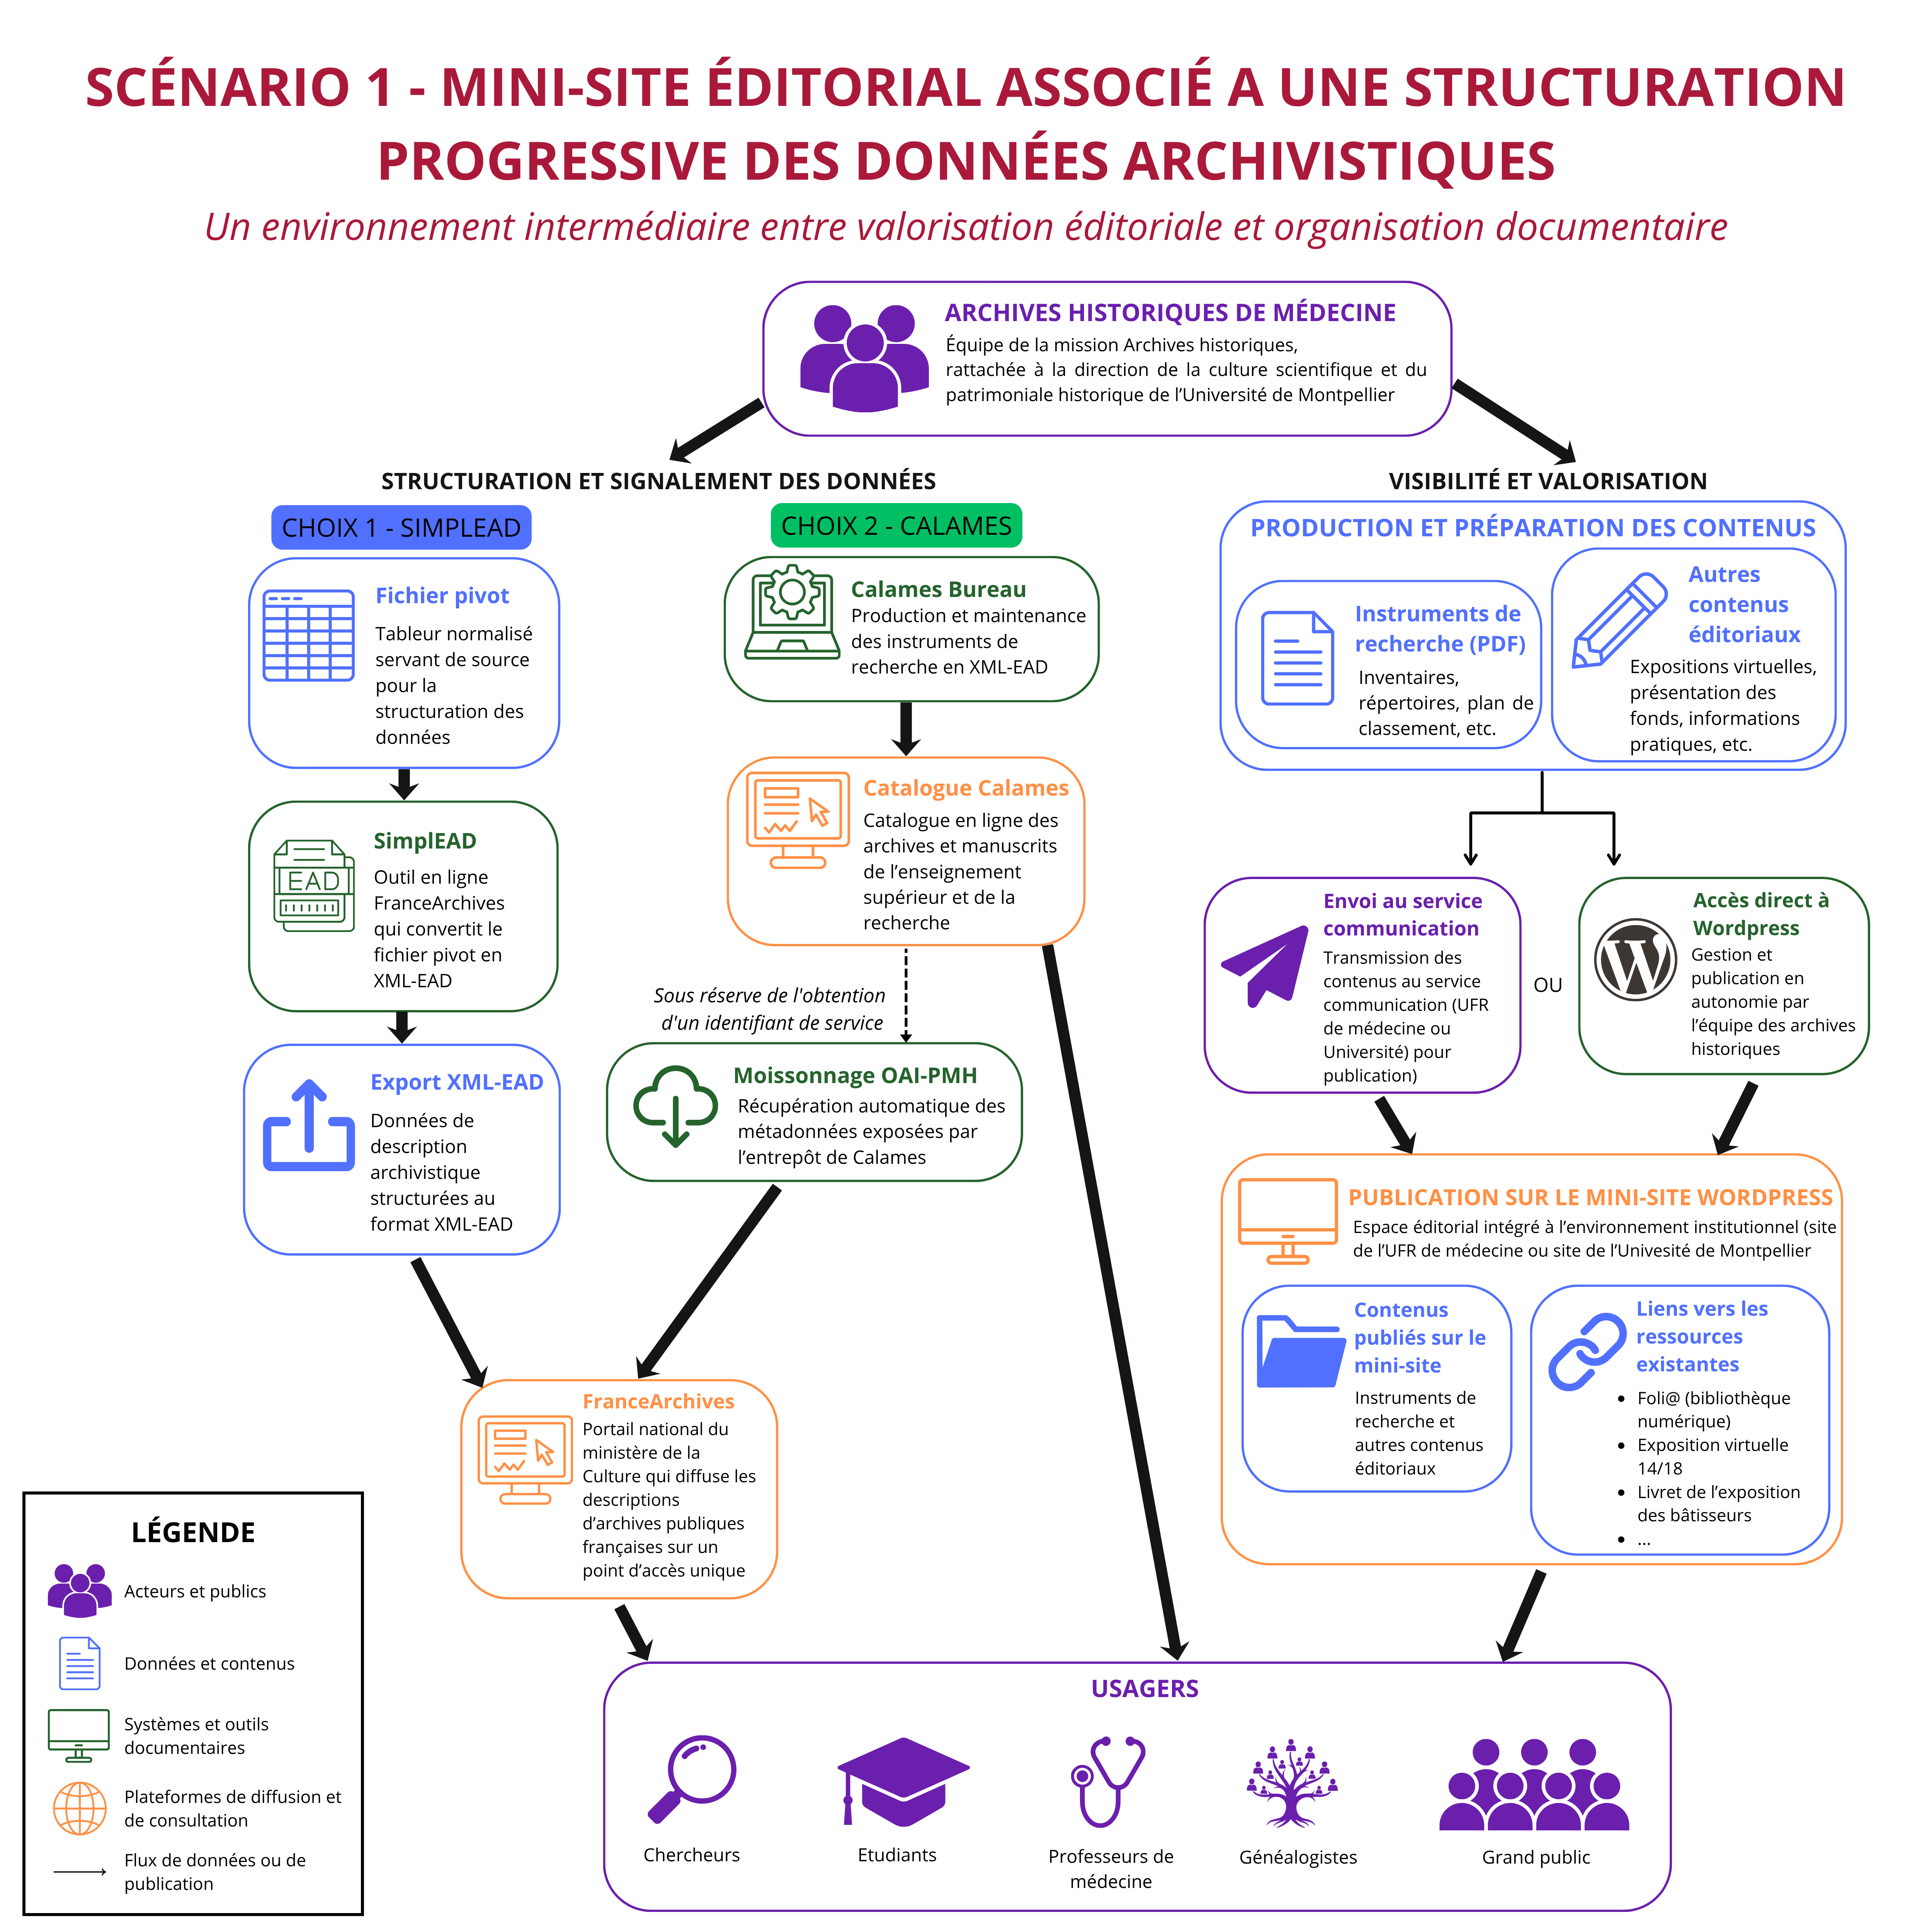
\includegraphics[
		width=\linewidth,
		height=1\textheight,
		keepaspectratio
		]{images/scenario1.png}
		\caption{Scénarios de structuration et de signalement des instruments de recherche et articulation avec le mini-site institutionnel}
		\label{fig:scenario1}
	\end{figure}
\end{landscape}

\chapter{Articulation des descriptions archivistiques et des reproductions numériques}
\label{chap:articulation-descriptions-reproductions}
\chapitrecourt{Descriptions et reproductions numériques}

La structuration et le \gls{signalement} des instruments de recherche ne constituent qu'une composante de la diffusion numérique des Archives historiques. La mise à disposition des reproductions exige également de déterminer où héberger les fichiers, comment les relier aux descriptions archivistiques et selon quelles modalités les rendre consultables. Production des descriptions, conservation des fichiers, exposition technique des images et restitution à l'usager peuvent ainsi relever de composants distincts.

Les essais conduits dans WordPress ont d'abord précisé les besoins auxquels un simple \gls{cms} ne répond pas. L'étude de Foli@ fournit ensuite un retour d'expérience sur une architecture associant gestion documentaire, \glspl{api}, services \gls{iiif} et visionneuse. À partir de ce modèle, le chapitre évalue les possibilités offertes par Flora, déjà acquis par l'Université, puis l'intérêt de Nakala comme entrepôt alternatif ou complémentaire pour les reproductions.


\section{Les besoins de consultation mis en évidence par le mini-site}
\label{sec:limites-cms-diffusion-documentaire}

\subsection{Les limites de la galerie et de l'affichage agrandi}

L'expérimentation conduite dans l'environnement WordPress de préproduction confirme les limites du \gls{cms} pour la diffusion documentaire. Pour restituer le \enquote{musée des archives}, les vingt-deux pièces sélectionnées ont d'abord été réunies au moyen du bloc \emph{Gallery}, qui permet d'afficher plusieurs images sous la forme d'une galerie et d'en paramétrer la disposition\footcite{WordPressGalleryBlock}. Sur la page générale, les reproductions apparaissent toutefois comme une succession de vignettes de petites dimensions (fig.~\ref{fig:musee-archives-wordpress-galerie}), ce qui donne une vue d'ensemble de la sélection mais uniformise des documents de formats et de natures différents et rend leur identification difficile lorsque les légendes sont longues.

\begin{figure}[htbp]
	\centering
	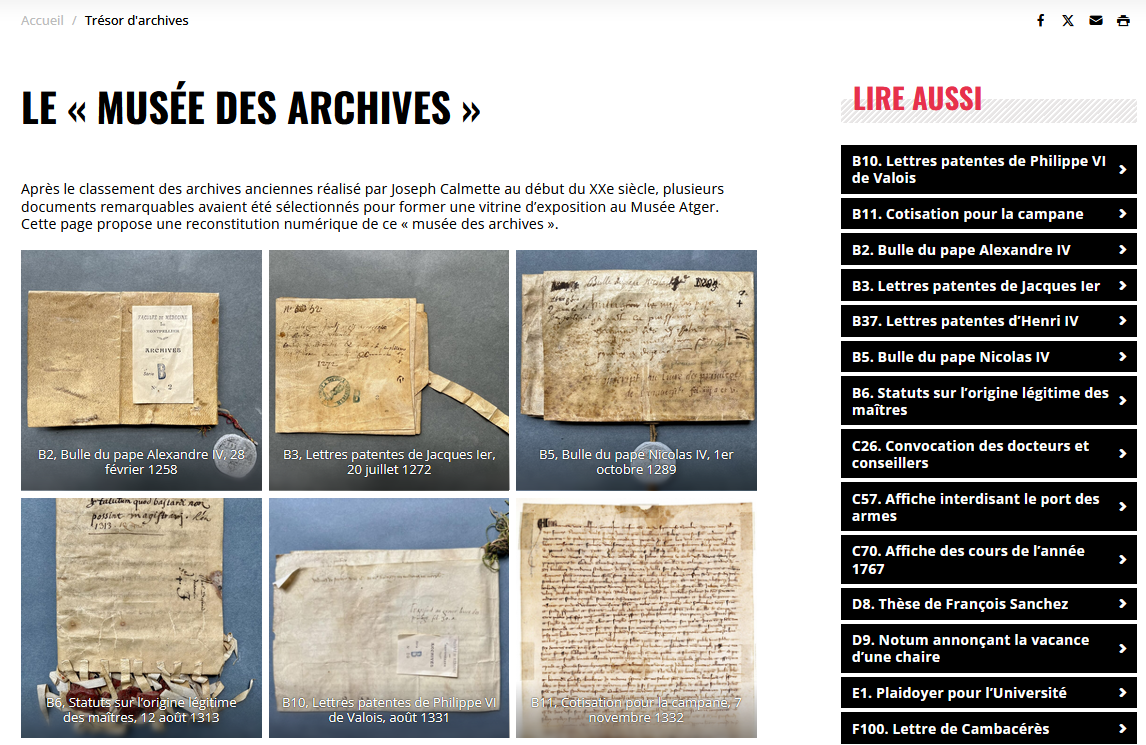
\includegraphics[width=0.92\textwidth]{images/museearchives_um_1.png}
	\caption[Présentation générale du \enquote{musée des archives} dans WordPress]
	{Présentation générale du \enquote{musée des archives} dans l'environnement WordPress de préproduction de l'Université de Montpellier : les reproductions et leurs légendes sont disposées sous la forme d'une succession de vignettes. Capture d'écran et redimensionnement : Clara Martin, août 2026}
	\label{fig:musee-archives-wordpress-galerie}
\end{figure}

L'ouverture d'une image déclenche un affichage agrandi en surimpression de la page (fig.~\ref{fig:musee-archives-wordpress-image}). Celui-ci conserve la légende associée au fichier, mais ne propose ni agrandissement progressif, ni déplacement dans l'image, ni sélection d'une zone précise. Peu gênante pour une illustration, cette limitation empêche l'examen détaillé de manuscrits, de registres ou de pièces de grand format.

\begin{figure}[htbp]
	\centering
	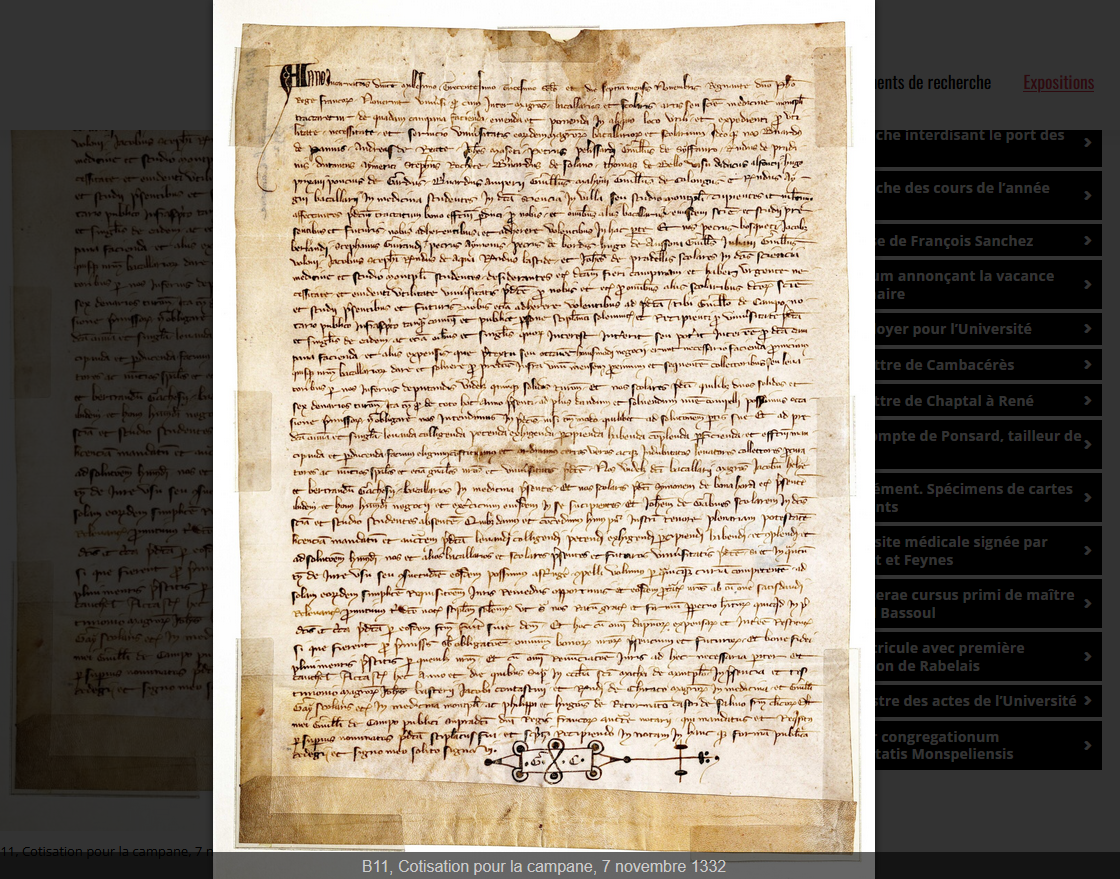
\includegraphics[
	width=0.78\textwidth,
	height=0.68\textheight,
	keepaspectratio
	]{images/museearchives_um_2.png}
	\caption[Affichage agrandi d'une reproduction dans WordPress]
	{Affichage agrandi de la pièce \texttt{B11}, \emph{Cotisation pour la campane}, dans l'environnement WordPress de préproduction : la légende demeure visible, mais l'image ne peut être ni agrandie ni déplacée. Capture d'écran et redimensionnement : Clara Martin, août 2026}
	\label{fig:musee-archives-wordpress-image}
\end{figure}

Lorsque plusieurs reproductions sont réunies sur une même page, des flèches latérales permettent de passer de l'une à l'autre, mais la légende disparaît dans la configuration testée (fig.~\ref{fig:musee-archives-wordpress-navigation}). La reproduction se trouve alors dissociée de sa cote, de son intitulé et de son analyse, comme sur la page consacrée aux trois spécimens de cartes d'étudiants de la série \enquote{Q Supplément}\footnote{Cette disparition ne constitue pas une impossibilité technique propre à WordPress, mais une limite du fonctionnement actuel de son dispositif d'agrandissement. Le problème est recensé dans le dépôt de développement de Gutenberg depuis 2024 : les légendes sont masquées dans la vue agrandie depuis WordPress 6.5 (\cite{WordPressGutenbergIssue60469}). Une proposition de modification ouverte en août 2026 prévoit d'afficher la légende correspondant à chaque image et de l'actualiser pendant la navigation au sein d'une galerie (\cite{WordPressGutenbergPR81500}). Une évolution du logiciel ou un développement spécifique du composant employé par l'Université pourrait donc corriger ce comportement, sous réserve des contraintes de maintenance de l'environnement institutionnel.}.

\begin{figure}[htbp]
	\centering
	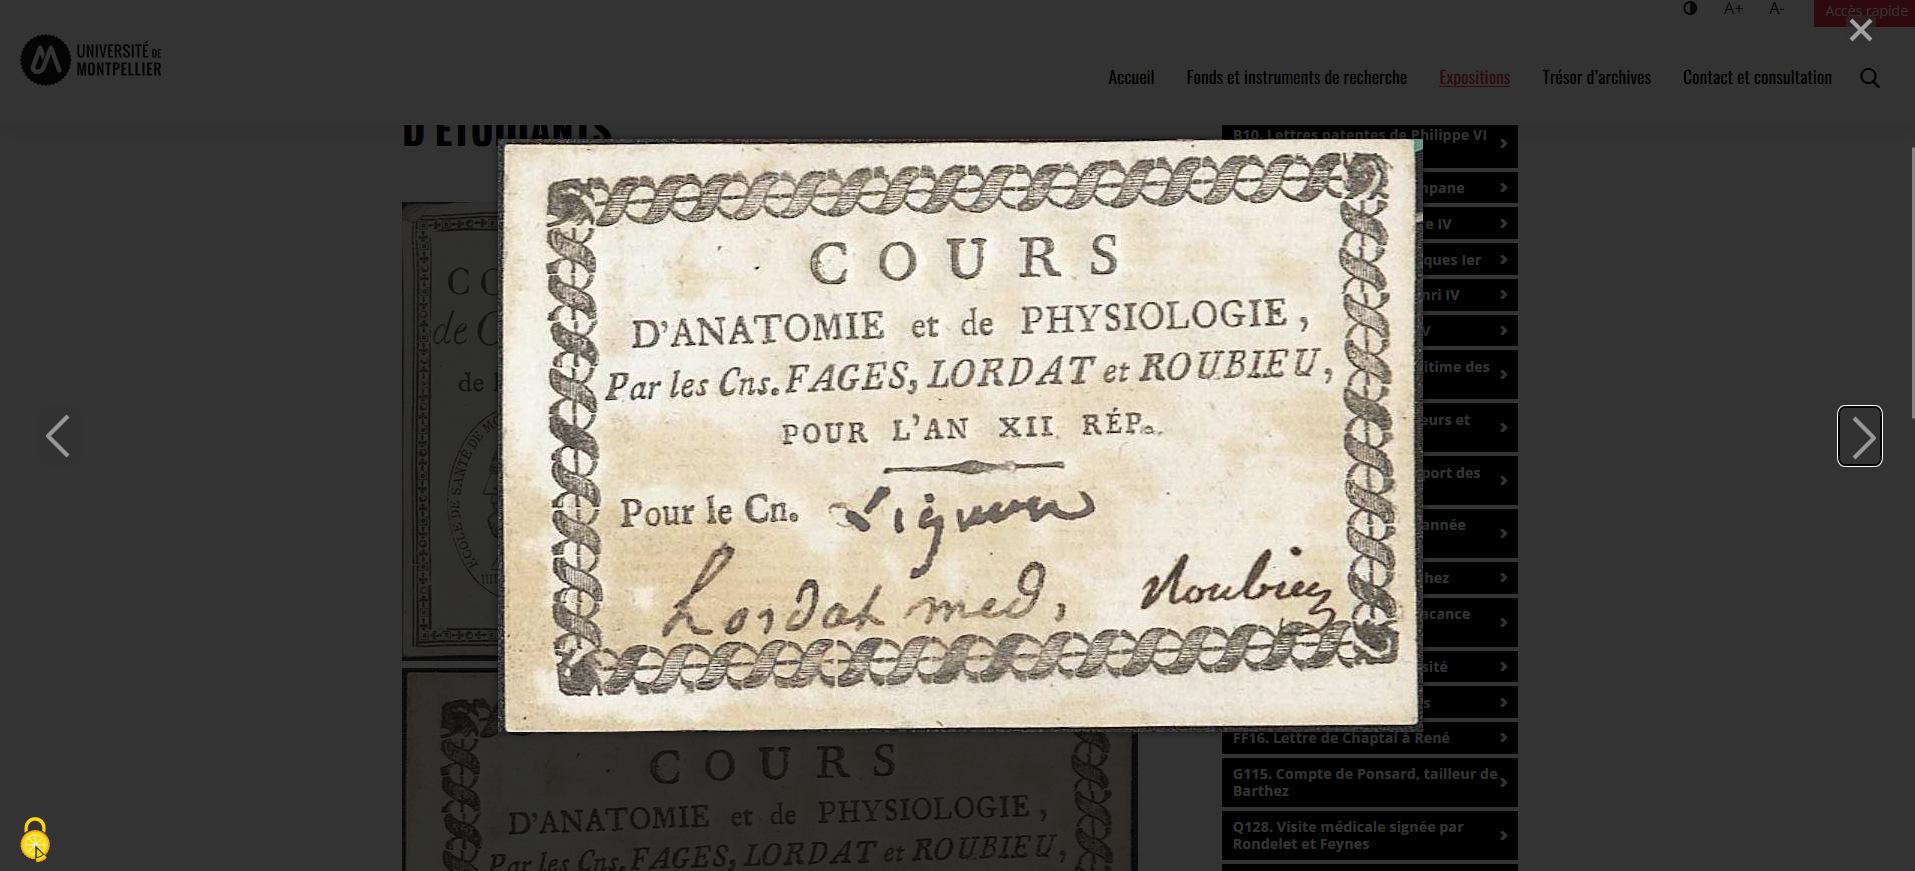
\includegraphics[width=\textwidth]{images/museearchives_um_3.png}
	\caption[Navigation entre plusieurs reproductions dépourvues de légende]
	{Navigation entre les trois reproductions réunies sur la page \enquote{Q Supplément. Spécimens de cartes d'étudiants} : les flèches permettent de passer d'une image à l'autre, mais la légende n'est plus affichée dans l'environnement WordPress testé. Capture d'écran et redimensionnement : Clara Martin, août 2026}
	\label{fig:musee-archives-wordpress-navigation}
\end{figure}

Ces essais ont conduit à utiliser la page générale du \enquote{musée des archives}, également accessible depuis la rubrique consacrée aux expositions, comme sommaire visuel : chaque vignette renvoie vers une page propre au document. Cette organisation alourdit la structure éditoriale, mais maintient l'association entre reproduction, cote, intitulé, date et texte de présentation ; elle ne remédie toutefois pas aux limites de consultation de l'image elle-même.


\subsection{Séparer la médiation des ressources documentaires}

La médiathèque WordPress permet de téléverser et de gérer les images, documents, fichiers audio et vidéo employés dans les contenus du site\footcite{WordPressMediaLibrary}. La taille maximale des fichiers dépend cependant de la configuration de l'hébergement, notamment des paramètres définis au niveau du serveur\footcite{WordPressMaxUploadSize}. Le volume des corpus, la définition nécessaire à leur examen et le besoin de réutiliser les objets numériques dans plusieurs interfaces excluent donc d'en faire le réservoir principal des images patrimoniales.

La même séparation vaut pour les descriptions : reproduire dans WordPress le contenu détaillé des instruments de recherche créerait une seconde version des données dont les corrections devraient être reportées dans plusieurs environnements. Le mini-site doit donc conserver des présentations synthétiques et renvoyer vers les descriptions structurées et les reproductions administrées ailleurs.


\subsection{Les conditions juridiques de la diffusion}

La mise en ligne ne peut être déduite de la seule communicabilité : la consultation d'un document dans un cadre contrôlé se distingue de sa diffusion publique, potentiellement indexable par les moteurs de recherche et accessible sans limitation, notamment lorsqu'il contient des données personnelles\footcite[pp.~99--101]{MalletPoujol2009}. Pour les fonds photographiques ou sonores, la détention du support doit en outre être distinguée des droits autorisant son exploitation ; selon les documents, la publication peut engager les droits de l'auteur ainsi que ceux des personnes ou des œuvres représentées\footcite[pp.~71--76]{Dieuzeide1998}. Chaque corpus devra donc faire l'objet d'une analyse précisant le statut juridique des documents, les titulaires et l'étendue des droits cédés, la présence éventuelle de données protégées, les crédits obligatoires et les conditions de consultation ou de réutilisation des fichiers.

L'expérimentation délimite ainsi le rôle du mini-site : assurer la médiation et organiser l'accès aux ressources, tandis que leur administration et leur consultation approfondie relèvent d'outils spécialisés. Foli@ fournit à l'échelle montpelliéraine un exemple de cette répartition fonctionnelle.


\section{Foli@ : l'évolution d'une bibliothèque numérique patrimoniale universitaire}
\label{sec:retour-experience-folia}

Foli@ est la bibliothèque numérique publique d'un environnement construit autour de Flora, progiciel web de gestion et de valorisation des collections patrimoniales permettant de centraliser données descriptives, données de gestion et ressources numériques\footcite{FloraLogicielGestion}. Son évolution fournit un retour d'expérience local sur l'organisation technique nécessaire à l'administration, à la diffusion et à la consultation de collections numérisées. Il ne s'agit pas d'en reproduire l'infrastructure pour les Archives historiques, mais d'en comprendre l'\gls{architecture-documentaire}\footnote{La politique patrimoniale du \gls{scdi} et ses projets transversaux seront examinés dans la partie~\ref{part:ecosysteme-patrimonial}.}.


\subsection{De la gestion des corpus à leur diffusion dans plusieurs réseaux}

Les universités montpelliéraines disposent avec Foli@ d'une bibliothèque numérique patrimoniale dont la numérisation et la diffusion sont assurées par le \gls{scdi}\footcite{SCDIFolia}. Créé en 2021 lors de la réorganisation consécutive à la fin de la Bibliothèque interuniversitaire de Montpellier, celui-ci exerce notamment des missions de coopération en matière d'informatique documentaire et de patrimoine écrit\footcite{SCDI2021}. Foli@ rassemble plus de 6\,500 documents numérisés répartis en neuf corpus thématiques : manuscrits médiévaux, imprimés anciens du XV\textsuperscript{e} au XIX\textsuperscript{e} siècle relatifs notamment à l'histoire de la médecine, de la pharmacie et de la botanique, cartes et plans, vues d'optique ou documents consacrés aux arts du cirque\footcite{Vanjak2026}.

Leur gestion repose sur Flora, employé par le \gls{scdi} depuis la fin des années 2000. Le logiciel administre les \glspl{metadonnees}, les fichiers numériques et les relations entre les notices, les reproductions, leur pagination et leur ordre de consultation\footnote{Entretiens avec Hélène Lorblanchet, Marie Nikichine, Audrey Cogoluègnès et Guenno Marti, Service de coopération documentaire interuniversitaire de Montpellier, 12 mai 2026, et avec Audrey Cogoluègnès, Marie Nikichine, Guenno Marti et Sébastien Leyreloup, 10 juillet 2026.}. Également employé pour les thèses de doctorat, les thèses d'exercice et les mémoires, Flora a été adapté aux collections patrimoniales par une modification du back-office au début des années 2010, puis par l'ajout de tables et de champs spécifiques à partir de 2014.

Foli@ complète plusieurs dispositifs de \gls{signalement} : ses ressources sont, dans leur quasi-totalité, également accessibles depuis le catalogue des bibliothèques universitaires de Montpellier, le Sudoc, Calames, Gallica ou Isidore\footcite{Vanjak2026}. Certaines notices de Calames renvoient ainsi vers une numérisation consultable dans Foli@. La refonte mise en production en juin 2026 accentue cette circulation entre plusieurs environnements en séparant l'administration des ressources de leur restitution publique.


\subsection{La refonte de 2026 : séparer gestion documentaire, interface publique et visionneuse}

\paragraph{Du portail Flora à une interface Drupal distincte}

Jusqu'en juin 2026, Foli@ était diffusée au moyen du portail public de Flora, qui assurait à la fois une fonction de \gls{ged}, par l'administration des fichiers et de leurs \glspl{metadonnees}, et leur restitution publique. Les collections étaient présentées selon une logique proche de celle d'un catalogue, sous forme de listes de résultats, de facettes et de vignettes. Certaines images apparaissaient comme des résultats individualisés, accompagnées d'informations sur le document auquel elles appartenaient, sa cote, sa date, le folio concerné ou les caractéristiques de la reproduction (fig.~\ref{fig:folia-ancienne-interface}).

\begin{figure}[htbp]
	\centering
	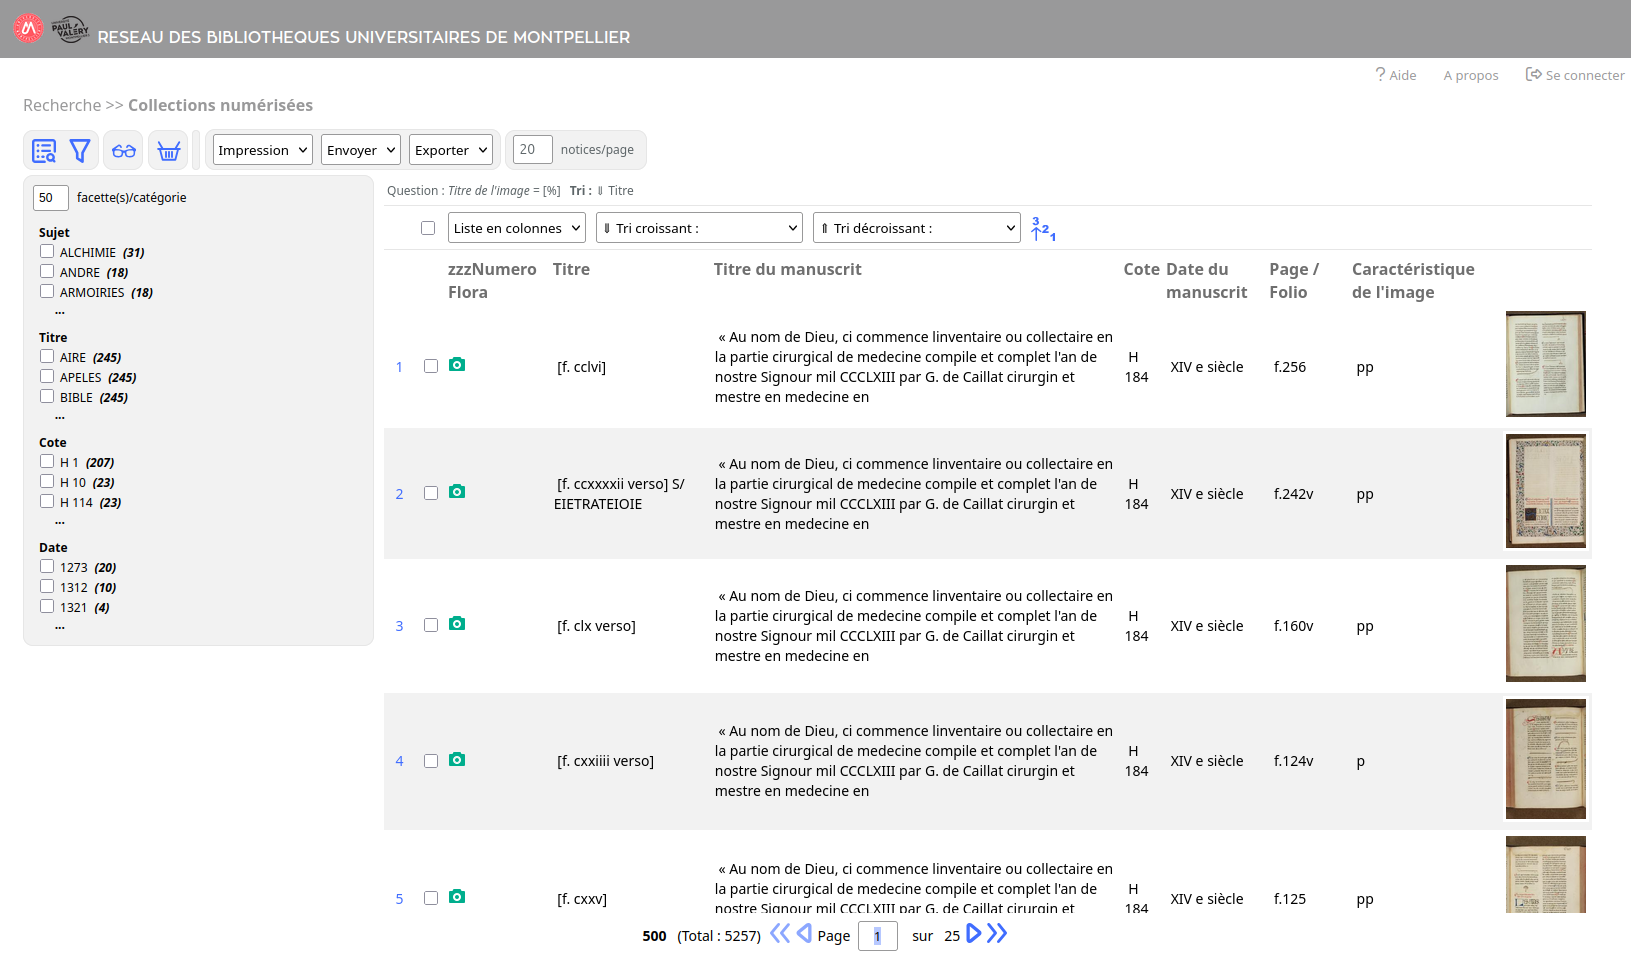
\includegraphics[
	width=\textwidth,
	height=0.72\textheight,
	keepaspectratio
	]{images/folia_ancienne_interface.png}
	\caption{Ancienne interface de diffusion des collections numérisées dans le portail Flora : affichage d'images sous forme de liste de résultats. Capture d'écran recadrée afin de rendre lisible la zone de l'interface concernée}
	\label{fig:folia-ancienne-interface}
\end{figure}

À l'échelle d'un document, la visionneuse native permettait de parcourir les reproductions dans l'ordre enregistré dans Flora. Les relations entre document, images, pagination et séquence existaient donc déjà dans le modèle documentaire, mais leur restitution demeurait liée à son interface.

Le rapport d'activité de 2021 décrit encore une chaîne dans laquelle les documents étaient numérisés, chargés dans la \gls{ged} Flora, sauvegardés puis mis en ligne dans Foli@, parallèlement à la préparation des \glspl{metadonnees} destinées au logiciel\footcite{SCDI2021}. Le plan d'action pour 2023 distingue ensuite l'intégration de nouveaux corpus, l'évolution de l'interface de Foli@ et l'archivage de la \gls{ged}, faisant apparaître une évolution séparée de l'environnement de gestion et de sa restitution publique\footcite{SCDI2022}.

Cette évolution aboutit en juin 2026 à une nouvelle instance de Foli@ : les corpus, leurs \glspl{metadonnees} et leurs fichiers demeurent administrés dans Flora, tandis qu'un site distinct développé sous \gls{drupal} assure leur diffusion\footcite{Vanjak2026}. Ce \gls{cms} permet au \gls{scdi} de faire évoluer la navigation et les contenus éditoriaux sans remplacer le socle documentaire. La page d'accueil associe ainsi moteur de recherche, accès aux corpus, actualités, contenus de présentation et informations sur la bibliothèque numérique (fig.~\ref{fig:folia-nouvelle-accueil}).

\begin{figure}[htbp]
	\centering
	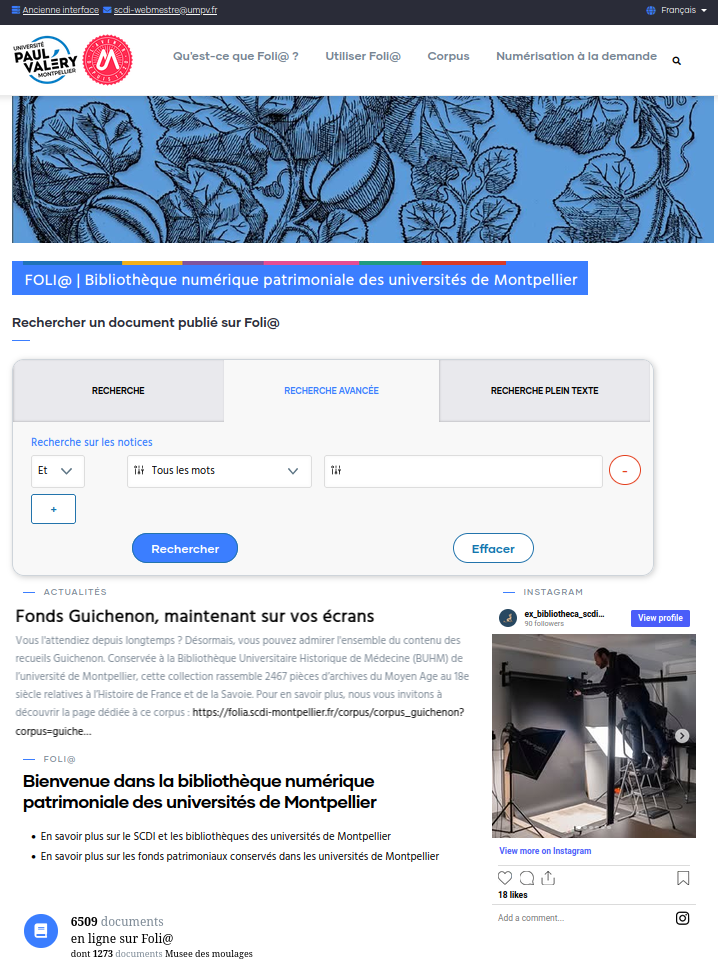
\includegraphics[
	width=0.72\textwidth,
	height=0.72\textheight,
	keepaspectratio
	]{images/folia_nouvelle_interface_1.png}
	\caption{Page d'accueil de la nouvelle interface de Foli@ mise en production en juin 2026. Capture d'écran recadrée afin de rendre lisible la zone de l'interface concernée}
	\label{fig:folia-nouvelle-accueil}
\end{figure}

L'aide distingue une recherche simple ou avancée sur les \glspl{metadonnees}, une recherche en plein texte dans les imprimés numérisés et une recherche par corpus à partir d'index dédiés. Les résultats peuvent être affinés par auteurs, corpus, dates, types documentaires, sujets ou localisations ; chaque entrée regroupe le titre, la date, la cote, le lieu de conservation et le type documentaire (fig.~\ref{fig:folia-nouvelle-resultats}).

\begin{figure}[htbp]
	\centering
	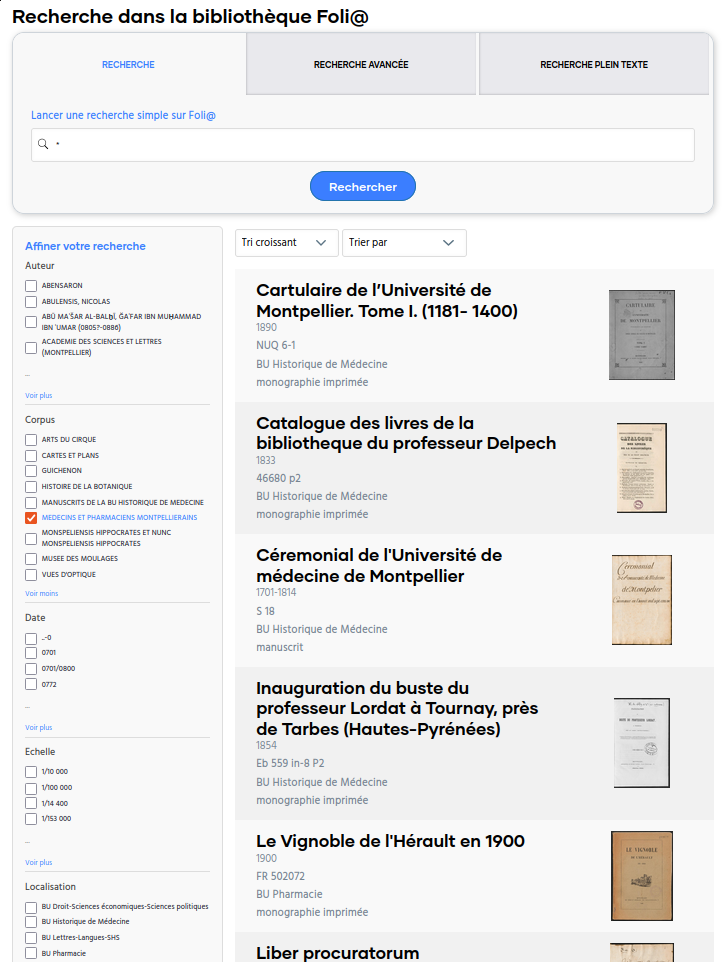
\includegraphics[
	width=\textwidth,
	height=0.72\textheight,
	keepaspectratio
	]{images/folia_nouvelle_interface_2.png}
	\caption{Affichage des résultats de recherche dans la nouvelle interface de Foli@ mise en production en juin 2026. Capture d'écran recadrée afin de rendre lisible la zone de l'interface concernée}
	\label{fig:folia-nouvelle-resultats}
\end{figure}

La consultation des reproductions est quant à elle confiée à \gls{mirador}, selon les standards \gls{iiif}. La nouvelle Foli@ répartit donc entre Flora, \gls{drupal} et \gls{mirador} les fonctions auparavant plus étroitement réunies.


\subsection{IIIF et Mirador : exposer, structurer et restituer les reproductions}

La séparation observée dans Foli@ correspond au problème auquel \gls{iiif} a été conçu pour répondre. Les bibliothèques numériques ont longtemps associé étroitement dépôts d'images, serveurs et applications de consultation, créant des environnements propres à chaque institution et limitant la réutilisation des ressources\footcite{SnydmanSandersonCramer2015}. Les \glspl{api} communes de \gls{iiif} permettent au contraire de rendre les images et les informations nécessaires à leur présentation accessibles à plusieurs applications sans déplacer les fichiers vers chacune d'elles.

Cette logique est mise en œuvre selon des modalités différentes dans les bibliothèques universitaires. À l'université Johns Hopkins, la \emph{Digital Library of Medieval Manuscripts} préexistante a été adaptée pour intégrer des visionneuses compatibles avec \gls{iiif} sans remplacer l'ensemble de son infrastructure ; à Harvard, les objets des collections numériques sont associés à des \glspl{manifeste-iiif} ouvrables dans différentes visionneuses et réutilisables dans d'autres environnements\footcite{ChenZhang2021IIIF}.

\paragraph{L'Image API : exposer les fichiers}

L'\emph{IIIF Image API} agit au niveau du fichier image. Un serveur compatible lui associe un identifiant et répond à des \glspl{uri} normalisés dont les paramètres indiquent la région demandée, ses dimensions, son orientation, sa qualité et son format\footcite{IIIFImageAPI}\footcite{SnydmanSandersonCramer2015}. Une visionneuse peut ainsi obtenir l'image entière ou seulement la portion et la résolution nécessaires à l'affichage : l'\gls{interoperabilite} porte ici sur l'accès technique à la ressource graphique.

\paragraph{La Presentation API : organiser les vues}

L'\emph{IIIF Presentation API} décrit dans un \gls{manifeste-iiif}, structuré en \gls{jsonld}, les \glspl{metadonnees} nécessaires à la présentation d'un objet et l'organisation de ses différentes vues\footcite{IIIFPresentationAPI}. Chaque page ou surface peut être représentée par un \emph{Canvas} auquel est associée sa reproduction : un registre numérisé page à page peut ainsi être restitué comme un objet ordonné plutôt que comme une juxtaposition de fichiers.

Cette fonction peut exploiter des relations déjà enregistrées dans le système documentaire. Dans Foli@, Flora connaissait avant l'adoption de \gls{iiif} l'appartenance des images à un document, leur pagination et leur ordre ; la \emph{Presentation API} permet désormais d'exprimer ces informations dans une ressource interprétable par d'autres applications. Elle ne remplace pas pour autant les standards de description documentaire : les descriptions plus riches peuvent demeurer dans leurs systèmes propres\footcite{SnydmanSandersonCramer2015}. Dans le domaine des archives, une expérimentation menée sur des fonds audiovisuels a ainsi montré que les objets \emph{Collection}, \emph{Manifest} et \emph{Canvas} peuvent correspondre à différents niveaux d'une structure archivistique et être reliés à une description en \gls{ead}\footcite{Critelli2026IIIFArchives}.

\paragraph{Mirador : interpréter les manifestes}

\gls{mirador} est une visionneuse web libre capable d'interpréter les \glspl{manifeste-iiif}, d'en restituer les vues et d'exploiter leurs structures de navigation\footcite{Mirador}. Conçue comme une application JavaScript configurable et extensible, elle peut être intégrée à une plateforme existante et afficher des ressources provenant de plusieurs environnements compatibles avec \gls{iiif}\footcite{WolffProbstBodenschatz2024}. La matrice maintenue par le consortium \gls{iiif} permet de vérifier la prise en charge par les différentes visionneuses des fonctionnalités de la \emph{Presentation API}\footcite{IIIFViewerMatrix3}, tandis que le \emph{IIIF Cookbook} fournit des exemples d'implémentation documentés pour construire et vérifier les \glspl{manifeste-iiif}\footcite{IIIFCookbook}.

FranceArchives exploite cette indépendance entre ressource et visionneuse pour intégrer dans ses notices des images \gls{iiif} hébergées par des services partenaires : les reproductions sont consultables dans \gls{mirador} ou Universal Viewer, tandis que leur contexte descriptif et le renvoi vers le site d'origine sont conservés\footcite{FranceArchivesIIIF2026}. Les recommandations élaborées avec Biblissima+ prévoient notamment des \glspl{uri} standardisés et pérennes pour les \glspl{manifeste-iiif} et les autres ressources \gls{iiif}, afin de permettre leur appel par des applications tierces\footcite{BiblissimaFranceArchivesIIIF2023}. Le mode multifenêtre de \gls{mirador} permet en outre de comparer des documents provenant d'un même fonds, de fonds différents ou d'institutions distinctes\footcite{FranceArchivesIIIF2026}.

Dans la nouvelle Foli@, \gls{drupal} appelle ainsi \gls{mirador}, tandis qu'un générateur développé autour de Flora produit les \glspl{manifeste-iiif} nécessaires à la consultation\footcite{Vanjak2026}\footnote{Échanges avec Audrey Cogoluègnès, Marie Nikichine, Guenno Marti et Sébastien Leyreloup, Service de coopération documentaire interuniversitaire de Montpellier, 10 juillet 2026.}.


\subsection{Les flux de données entre Flora et les autres systèmes}

La nouvelle architecture mobilise plusieurs mécanismes d'échange correspondant à des destinations distinctes. Pour alimenter \gls{drupal}, Flora expose des données par ses \glspl{api} \gls{rest}\footnote{Échanges avec Audrey Cogoluègnès, Marie Nikichine, Guenno Marti et Sébastien Leyreloup, Service de coopération documentaire interuniversitaire de Montpellier, 10 juillet 2026.}. Une \gls{api} est une interface par laquelle une application rend certaines de ses données ou fonctions accessibles à d'autres applications\footcite{CNILAPI}. \gls{rest}, pour \emph{Representational State Transfer}, désigne un style d'architecture appliqué aux services web : les ressources sont identifiées par des \glspl{uri}, interrogées au moyen du protocole \gls{http} et renvoyées sous une représentation qui peut notamment être encodée en \gls{json}\footcite{Fielding2000REST}. \gls{drupal} peut ainsi recevoir les \glspl{metadonnees} nécessaires à l'affichage sans accéder directement à la base interne du progiciel.

D'autres flux relient Flora aux réseaux documentaires : \gls{z3950}, protocole client--serveur normalisé pour l'interrogation de systèmes documentaires distants, assure les échanges avec le Sudoc\footcite{Lynch1997Z3950}, tandis que \gls{oaipmh} permet à un entrepôt d'exposer des lots de \glspl{metadonnees} récupérés périodiquement par un moissonneur et sert ici au \gls{signalement} dans Gallica\footcite{OAIPMH2002}\footnote{Entretien avec Hélène Lorblanchet, Marie Nikichine, Audrey Cogoluègnès et Guenno Marti, Service de coopération documentaire interuniversitaire de Montpellier, 12 mai 2026.}. Les services \gls{iiif}, examinés précédemment, assurent pour leur part l'exposition et la restitution des reproductions.

Le schéma élaboré par le \gls{scdi} replace ces différents flux dans l'environnement général de Flora (fig.~\ref{fig:schema-folia}). L'interface publique constitue ainsi l'aboutissement d'échanges entre plusieurs composants plutôt que le lieu où l'ensemble des données est stocké et administré.

\begin{figure}[htbp]
	\centering
	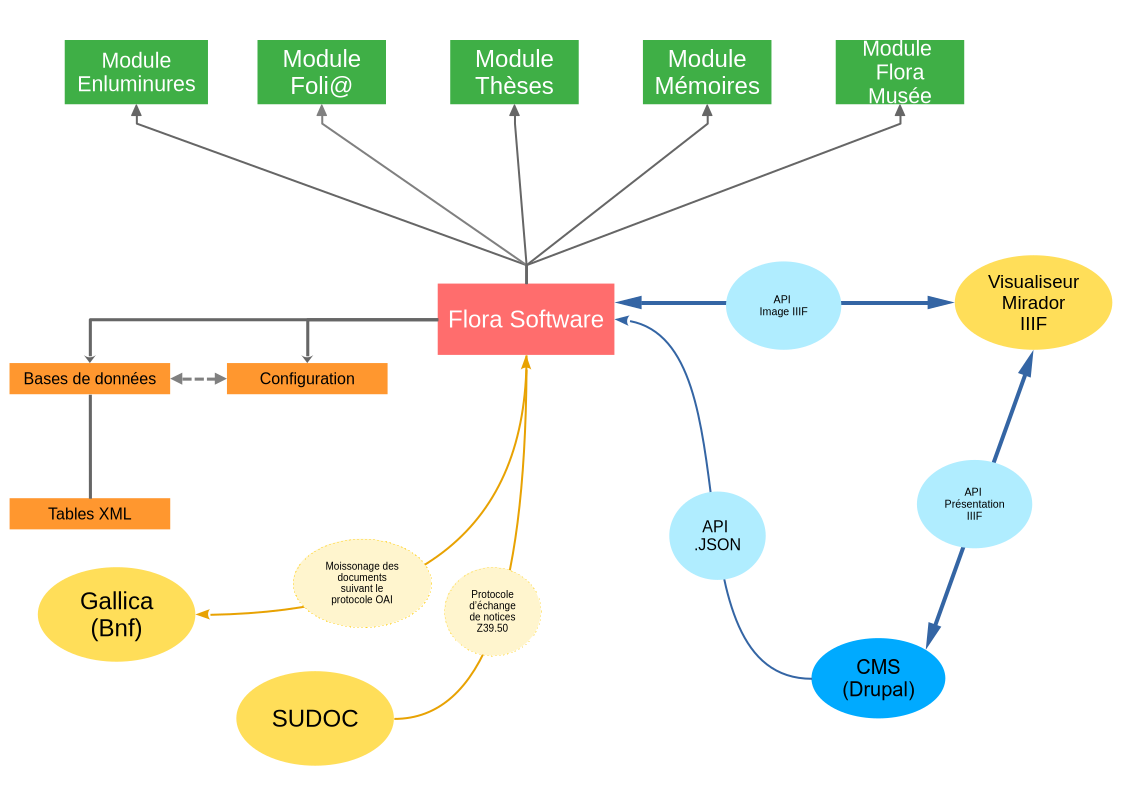
\includegraphics[
	width=\textwidth,
	height=0.78\textheight,
	keepaspectratio
	]{images/schema_folia.png}
	\caption{Architecture et flux de données de la nouvelle instance de Foli@ mise en production en juin 2026. Schéma élaboré par le Service de coopération documentaire interuniversitaire de Montpellier.}
	\label{fig:schema-folia}
\end{figure}


\subsection{Les développements propres à Foli@ : les limites d'une transposition aux archives}

Cette \gls{architecture-documentaire} résulte toutefois d'une construction progressive dans laquelle les fonctions standards de Flora ont été complétées par des paramétrages et des développements propres au \gls{scdi}\footnote{Échanges avec Audrey Cogoluègnès, Marie Nikichine, Guenno Marti et Sébastien Leyreloup, Service de coopération documentaire interuniversitaire de Montpellier, 10 juillet 2026.}. Dès 2014, des tables de concordance, de pagination et de granularité ainsi que des champs complémentaires ont été ajoutés pour structurer les relations entre notices et reproductions. Les images ne disposent pas de notices iconographiques autonomes : une table conserve principalement leur identifiant technique et leur numéro de page, tandis que d'autres établissent leur ordre et leur rattachement au document\footnote{Ibid.}. Antérieurs à l'adoption de \gls{iiif}, ces développements fournissent aujourd'hui les informations structurelles nécessaires à la construction des \glspl{manifeste-iiif}.

Le modèle documentaire a lui aussi été adapté. Le module Musée repose sur la notion de \enquote{bien}, insuffisante pour restituer toutes les informations bibliographiques d'un livre ancien ; un développement articule donc certaines données issues du Sudoc avec celles du module. La refonte de 2026 a en outre nécessité l'enrichissement des \glspl{api} \gls{rest}, la création de vues \gls{json} adaptées à \gls{drupal} et le développement du générateur de \glspl{manifeste-iiif} associant images, \glspl{metadonnees} et informations structurelles\footnote{Ibid.}. Ces trois développements --- articulation bibliographique, enrichissement des \glspl{api} et production des \glspl{manifeste-iiif} --- ont représenté des coûts distincts et compliquent les montées de version ; en juillet 2026, le \gls{scdi} n'avait ainsi pas encore adopté Flora 4.7\footnote{Ibid.}.

Ce retour d'expérience invite à transposer le principe de l'architecture plutôt que son implémentation locale. Les fonctionnalités de Foli@ ne peuvent être présumées dans le module Archives de la nouvelle instance Flora acquise par l'Université ; leur évaluation doit donc porter sur ce que cette dernière fournit nativement et sur les éventuelles adaptations qu'exigerait son emploi pour les Archives historiques.


\section{L'évaluation de la nouvelle instance Flora pour les Archives historiques}
\label{sec:flora-architecture-documentaire}

L'étude de Foli@ conduit à examiner séparément deux fonctions décisives dans la nouvelle instance Flora acquise par l'Université : la réutilisation des descriptions archivistiques hors du progiciel et l'association puis l'exposition des reproductions numériques.


\subsection{Un environnement de gestion déjà acquis à l'échelle de l'Université}

La nouvelle instance était en cours de déploiement au moment du stage et ne doit pas être confondue avec celle qui soutient Foli@, fondée sur le module Musée et sur des développements accumulés depuis les années 2010\footnote{Échanges avec Audrey Cogoluègnès, Marie Nikichine, Guenno Marti et Sébastien Leyreloup, Service de coopération documentaire interuniversitaire de Montpellier, 10 juillet 2026.}. La diffusion des futures numérisations des Archives historiques n'étant pas appelée, à ce stade, à rejoindre Foli@, l'évaluation a porté sur les fonctionnalités standards et le paramétrage du nouveau déploiement.

\paragraph{Un projet destiné à fédérer des collections hétérogènes}

Le projet concerne des archives, des collections scientifiques, techniques et naturelles, des objets artistiques et mobiliers, des collections de recherche et des spécimens vivants, jusqu'alors administrés au moyen d'outils et d'espaces de stockage distincts\footnote{\emph{Réunion de lancement du projet}, Flora Software -- Université de Montpellier, 14 février 2025.}. Le cahier des charges visait donc un \enquote{logiciel commun de gestion des collections} prenant en charge les beaux-arts, les archives, les collections de muséum, scientifiques et techniques ainsi que leur valorisation publique\footnote{Ibid.}. Le périmètre associe notamment les collections des services centraux, de l'Institut des sciences de l'évolution de Montpellier et des facultés de pharmacie et de médecine ; les premières estimations atteignaient plusieurs dizaines de milliers de notices et plus de cent mille pour le seul ISEM\footnote{Ibid.}.

Cette mutualisation documentaire se retrouve dans la \gls{dcsph}, où le Service du patrimoine historique gère les collections patrimoniales et scientifiques, tandis que le Service des archives historiques, scientifiques et administratives prend en charge les archives\footnote{L'organisation de la \gls{dcsph} est présentée en annexe~\ref{annexe:dcSPH}.}.

\paragraph{Un périmètre fonctionnel associant collections et archives}

Le marché, notifié en décembre 2024 et lancé en février 2025, porte sur une licence site perpétuelle couvrant l'ensemble de l'Université et un nombre illimité d'utilisateurs\footnote{\emph{Planning prévisionnel du projet Flora -- Université de Montpellier}, version 4 du 17 mars 2026}. Flora regroupe quatre grandes familles fonctionnelles : gestion des collections, catalogage des bibliothèques, description et gestion des archives, gestion des documents et des ressources numériques\footcite{FloraLogicielGestion}. À ce socle peuvent s'ajouter des fonctions spécialisées, notamment la gestion des périodiques et de la circulation des documents, Flora-Archéo, Flora-ImmoPat, les services d'\gls{interoperabilite} par \gls{api} et \gls{oaipmh}, ainsi que la gestion archivistique avancée\footcite{FloraProfilRCIP2025}.

L'Université n'a pas acquis l'ensemble de ces extensions. Le marché porte principalement sur Flora Musée et sur le niveau avancé de Flora Archives ; l'offre comprend également un portail public reposant sur des composants WordPress\footnote{\emph{Présentation de l'offre Flora Software à l'Université de Montpellier}, audition de négociation, 18 juillet 2024.}. Le niveau 1 permet de saisir et de rechercher des fonds, des versements et des unités d'archives, de les organiser hiérarchiquement et de les relier aux autorités, aux thésaurus et aux autres entités documentaires\footcite{FloraCatalogueFormations2024}. Le niveau 2, acquis par l'Université, complète cette description par la gestion avancée des localisations et délocalisations, des magasins et unités de conditionnement, des éliminations, des utilisateurs, des réservations et des communications en salle de lecture\footcite{FloraCatalogueFormations2024}. Le même environnement peut ainsi administrer versements, unités d'archives, plans de classement, localisations, conditionnements, éliminations et communications\footnote{\emph{Réunion de lancement du projet}, Flora Software -- Université de Montpellier, 14 février 2025.}.

L'acquisition comprend enfin l'installation et le paramétrage de Flora et du portail, des environnements de test et de production, la reprise des données, des \glspl{referentiel} et des images, leur validation et les formations. La solution est hébergée \emph{on premise}, sur les serveurs de l'Université. La reprise repose sur deux fichiers pivots, l'un destiné aux collections et l'autre aux archives ; après une phase d'essai sur quatre bases, les autres ensembles et leurs images doivent être progressivement intégrés par l'Université\footnote{Ibid.}.

\paragraph{Une association tardive des Archives historiques qui transforme l'enjeu du stage}

Le déploiement s'étend de 2025 à 2026 : installation et paramétrage, élaboration et test des fichiers pivots, reprise d'un ensemble de données plus complet, validation des imports, puis mise en production\footnote{\emph{Planning prévisionnel du projet Flora -- Université de Montpellier}, version 4 du 17 mars 2026.}. La \enquote{recette} désigne ici la vérification de la reprise des données et de la conformité fonctionnelle de l'application avant son passage en production.

Le projet associe notamment la \gls{dcsph}, la \gls{dsin} et des référents documentaires\footnote{\emph{Réunion de lancement du projet}, Flora Software -- Université de Montpellier, 14 février 2025.}. Une formation à la reprise des données a été organisée en juin 2025, puis des sessions générales en janvier 2026, une formation au module Archives les 27 et 28 janvier et une formation à son administration au début du mois de février\footnote{\emph{Planning prévisionnel du projet Flora -- Université de Montpellier}, version 4 du 17 mars 2026.}.

Le suivi archivistique avait été confié à Manon Guillermin, chargée des archives courantes et intermédiaires. Les Archives historiques n'avaient été associées ni à la préparation du marché ni aux négociations qui en avaient déterminé le périmètre ; elles ont rejoint le projet alors que le logiciel était déjà acquis et paramétré\footnote{Réunion de travail avec Sophie Dikoff, Emma Bertrand, Manon Guillermin et Véronique Bourgade, 21 avril 2026.}. Le stage devait donc vérifier l'adéquation aux fonds historiques d'un environnement déjà retenu, plutôt que spécifier un nouvel outil.


\subsection{Produire dans Flora des descriptions réutilisables hors du logiciel : le test de l'export EAD}

Les fichiers, scripts et résultats de cette expérimentation sont documentés dans un dépôt GitHub.\footnote{Le dépôt, les données de test, les exports produits par Flora, les rapports de validation et le script de correction sont présentés en annexe~\ref{annexe:analyse-flora}.}

\paragraph{De la reprise des données à l'export EAD}

Le fichier pivot consacré aux unités d'archives prévoit notamment la cote de versement, le type d'entité, le cadre de classement, le numéro d'article et son unité parente, le service versant et le producteur, les dates, le titre et l'analyse, l'indexation, les supports, la communicabilité, les renvois et les fichiers numériques associés\footnote{Fichier pivot d'import des unités d'archives transmis dans le cadre du projet Flora, version utilisée par l'Université de Montpellier en 2026.}.

Le versement constitue le niveau d'entrée, tandis que les niveaux inférieurs relèvent de la catégorie générique des \enquote{unités d'archives}. Celles-ci peuvent être qualifiées comme groupe d'articles, article, dossier, sous-dossier ou pièce et reliées par des relations parent--enfant\footnote{\emph{Module Archives -- Descriptif fonctionnel}, Flora Software, 22 juillet 2024.}. Le modèle interne permet donc de représenter une arborescence de type \emph{versement > groupe d'articles > article > dossier > sous-dossier > pièce}, sans imposer l'emploi de tous ces niveaux.

Les premiers essais ont précisé les correspondances relatives à l'état de traitement, au support, à l'état matériel, à la communicabilité et aux identifiants\footnote{Réunion de travail avec Sophie Dikoff, Emma Bertrand, Manon Guillermin et Véronique Bourgade, 21 avril 2026.}. Le fichier pivot reste toutefois un format de reprise initiale : son import dépend de champs obligatoires, d'identifiants cohérents et de listes de valeurs contrôlées ; les notices peuvent ensuite être enrichies dans l'interface\footnote{\emph{Rapport d'analyse. Phase 2. Reprise des données (fichier pivot) Archives}, Flora Software, juillet 2026.}.

L'enjeu principal concernait leur réutilisation dans Calames ou FranceArchives. Le mémoire technique annonçait à cette fin un \enquote{export \gls{xml}-\gls{ead} pour les données d'archives}\footnote{\emph{Mémoire technique}, Decalog, version 3.0, 28 avril 2024, p.~18.}\footcite{Sibille2012}. L'évaluation a donc porté sur la conformité syntaxique des fichiers à l'\gls{ead} 2002 et sur la restitution des relations hiérarchiques définies dans Flora.

\paragraph{Un export mêlant des structures EAD 1998 et EAD 2002}

L'export a d'abord été testé sur une structure minimale à plat composée d'un versement et de trois articles, puis sur des descriptions enrichies et plusieurs arborescences\footnote{Tests de l'export \gls{xml}-\gls{ead} du module Archives de Flora réalisés dans le cadre du stage, printemps et été 2026.}.

Flora établit des correspondances avec plusieurs éléments spécialisés de l'\gls{ead} : \texttt{<origination>} pour le producteur, \texttt{<unitdate>} pour les dates, \texttt{<scopecontent>} pour l'analyse, \texttt{<accruals>} pour les accroissements, \texttt{<bibliography>} pour la bibliographie, \texttt{<odd>} pour les notes et \texttt{<physdesc>} pour le métrage. Le modèle interne contient donc une part importante des informations attendues dans un instrument de recherche.

Les fichiers exportés déclarent explicitement l'utilisation de la gls{dtd} \gls{ead} 2002 et ont donc été contrôlés contre celle-ci\footnote{Une DTD (\emph{Document Type Definition}) définit les éléments, attributs, relations hiérarchiques et modèles de contenu autorisés dans un document XML.}. Aucun des fichiers testés n'est cependant conforme à cette DTD ; le cas minimal à plat, c'est-à-dire un versement contenant trois articles directement rattachés, sans dossier, sous-dossier ni autre niveau hiérarchique intermédiaire, restitue correctement les trois unités et leurs identifiants sans duplication, mais produit déjà vingt-neuf erreurs de validation.

Une partie de ces écarts semble provenir d'un mélange entre des structures relevant de versions différentes de l'\gls{ead}. Les éléments \texttt{<admininfo>} et \texttt{<add>} appartiennent à la première version d'\gls{ead} publiée en 1998 mais ne figurent plus comme éléments dans la \gls{dtd} \gls{ead} 2002 pourtant déclarée par l'export. Leur présence suggère que le générateur conserve des structures héritées d'\gls{ead} 1998. L'élément \texttt{<unititle>} relève d'un problème différent : il n'est pas reconnu par la \gls{dtd} \gls{ead} 2002, qui attend \texttt{<unittitle>}.

D'autres erreurs concernent des éléments appartenant bien à \gls{ead} 2002 mais dont Flora ne respecte pas le modèle de contenu. Du texte ou des éléments sont placés directement dans \texttt{<otherfindaid>}, \texttt{<acqinfo>} et \texttt{<accessrestrict>} alors que la DTD attend une structuration interne déterminée ; certains blocs \texttt{<did>} ne contiennent en outre qu'un élément \texttt{<head>} sans les éléments descriptifs attendus.

\begin{table}[htbp]
	\centering
	\small
	\begin{tabular}{p{0.72\textwidth}r}
		\toprule
		\textbf{Principales erreurs du test minimal à plat} & \textbf{Occurrences} \\
		\midrule
		Contenu non structuré dans \texttt{<otherfindaid>} & 4 \\
		\texttt{<admininfo>} et \texttt{<add>} non reconnus & 4 + 4 \\
		Structure incorrecte de \texttt{<acqinfo>} & 4 \\
		Structure incorrecte de \texttt{<accessrestrict>} & 4 \\
		Bloc \texttt{<did>} insuffisamment structuré & 3 \\
		\texttt{<unititle>} au lieu de \texttt{<unittitle>} & 1 \\
		\bottomrule
	\end{tabular}
	\caption{Principales erreurs relevées lors de la validation de l'export EAD minimal à plat produit par Flora}
	\label{tab:flora-export-ead-minimal}
\end{table}

Les descriptions enrichies mobilisent davantage d'éléments spécialisés de l'\gls{ead}, notamment \texttt{<custodhist>}, \texttt{<appraisal>}, \texttt{<language>} et \texttt{<langusage>}, mais font apparaître de nouvelles erreurs de structure, notamment dans \texttt{<profiledesc>}, \texttt{<custodhist>} et \texttt{<appraisal>}\footnote{Ibid.}. Certaines informations de gestion sont également répétées entre le versement et ses unités enfants.

Les niveaux locaux sont exportés dans des composants \texttt{<c level="otherlevel">}. Cette syntaxe peut être valide si la valeur locale est correctement exprimée, mais son \gls{interoperabilite} dépend de la capacité de l'application destinataire à interpréter les niveaux propres à Flora.

\paragraph{Une restitution défectueuse des hiérarchies}

Les tests hiérarchiques ont révélé une anomalie distincte : une structure composée d'un article et de deux dossiers devait produire trois composants, mais en exportait cinq ; une arborescence à trois niveaux produisait six composants pour trois unités et deux branches article--dossier six composants pour quatre unités\footnote{Ibid.}. Chaque unité enfant est exportée comme composant autonome puis à nouveau sous son parent ; la duplication se cumule avec la profondeur et réemploie les mêmes identifiants à plusieurs emplacements.

L'anomalie porte ainsi sur la sérialisation des relations enregistrées dans Flora. Or la position d'une unité dans l'arborescence participe directement de son contexte archivistique : un fichier qui duplique les composants ne peut être transmis tel quel à une application destinataire, même si les notices individuelles sont correctement renseignées.

\paragraph{Une correction automatisée possible, mais non pérenne}

L'aplatissement des descriptions ou la multiplication des versements aurait limité les duplications au prix d'une perte de structure ; l'export simultané de plusieurs versements a par ailleurs produit une archive ZIP vide\footnote{Ibid.}. Ce comportement peut être propre à l'instance de préproduction testée, mais empêchait de retenir ce contournement.

Un script Python a été développé pour corriger le fichier minimal. Il remplace \texttt{<unititle>} par \texttt{<unittitle>}, supprime les enveloppes \texttt{<admininfo>} et \texttt{<add>} tout en conservant leur contenu, restructure \texttt{<otherfindaid>}, \texttt{<accessrestrict>} et \texttt{<acqinfo>} et complète les blocs \texttt{<did>} insuffisamment structurés\footnote{Test de correction automatisée de l'export \gls{xml}-\gls{ead} de Flora réalisé dans le cadre du stage, août 2026.}. Après transformation, le fichier minimal valide contre la \gls{dtd} \gls{ead} 2002, ce qui montre qu'une partie des anomalies suit des règles régulières pouvant être corrigées automatiquement.

Une telle transformation ne constitue toutefois pas une chaîne pérenne : il faudrait étendre les règles aux descriptions enrichies, reconstruire les hiérarchies, contrôler les valeurs locales et maintenir le script lors des évolutions de Flora. Le retour du \gls{scdi} montre précisément que les développements spécifiques doivent être testés lors des montées de version\footnote{Échanges avec Audrey Cogoluègnès, Marie Nikichine, Guenno Marti et Sébastien Leyreloup, Service de coopération documentaire interuniversitaire de Montpellier, 10 juillet 2026.}. Produire l'\gls{ead} à partir d'un export CSV, Excel ou \gls{json} déplacerait cette charge de transformation sans la supprimer\footnote{Point de travail avec Manon Guillermin sur Flora, 2 juin 2026.}.

La production de l'\gls{ead} a donc été dissociée des autres fonctions envisagées pour Flora, au profit d'outils dans lesquels ce format constitue directement le format de travail ou d'échange, notamment SimplEAD et Calames. Le constat reste circonscrit à l'instance de préproduction testée en 2026 : Flora permet de centraliser les données archivistiques, de les rechercher, d'établir des relations entre unités et d'associer de nombreux champs au vocabulaire \gls{ead}, mais aucun fichier contrôlé ne valide en l'état et les arborescences produisent des composants dupliqués.

L'export \gls{ead} figure dans la documentation contractuelle, mais aucun usage régulier n'a pu être identifié dans les retours recueillis. Ces résultats ne préjugent donc ni d'une correction ni d'une évolution ultérieure du logiciel ; ils établissent qu'au moment du test, l'instance disponible ne produisait pas une chaîne \gls{ead} directement exploitable pour un versement dans Calames ou un \gls{signalement} dans FranceArchives.

\paragraph{Le retour du Musée des Confluences : distinguer gestion locale et signalement national}

Le Musée des Confluences utilise Flora parce que le logiciel était déjà employé pour les collections, permettait de mutualiser les autorités et les thésaurus et offrait à une archiviste seule un environnement commun de centralisation. Les descriptions y sont largement organisées à plat et rattachées aux entrées ou aux versements ; les fonctions de recherche en plein texte et par autorités sont en revanche jugées satisfaisantes\footnote{Entretien avec Pauline Laugraud et Jérémie Léonard, Musée des Confluences de Lyon, 4 juin 2026.}. Le portail public permet d'associer aux notices des instruments de recherche sous forme de fichiers PDF joints\footnote{\emph{Portail des collections et des archives du Musée des Confluences}, rubrique Archives, consulté le 11 août 2026.}.

Cette organisation ne résout pas l'\gls{interoperabilite} : les échanges engagés avec FranceArchives n'ont pas abouti à une correspondance satisfaisante, les exports \gls{xml} ne constituent pas nécessairement des instruments \gls{ead} directement exploitables et le flux OAI en Dublin Core restitue les données à plat\footnote{Entretien avec Pauline Laugraud et Jérémie Léonard, Musée des Confluences de Lyon, 4 juin 2026.}. Ce retour confirme donc qu'un logiciel peut demeurer pertinent pour la gestion et la diffusion locale de notices sans constituer l'outil de production de l'instrument destiné au \gls{signalement} national.


\subsection{Associer les reproductions dans Flora et les exposer hors du logiciel}

L'échec de l'export \gls{ead} directement exploitable n'écarte pas Flora de l'\gls{architecture-documentaire}. Une seconde série de vérifications a porté sur sa capacité à administrer les reproductions et à les rendre accessibles à d'autres composants.

\paragraph{Associer les fichiers aux unités d'archives}

Flora 4.7 permet d'associer des fichiers, notamment JPEG et PDF, aux versements et aux unités d'archives et prévoit leur import. Le fichier pivot comporte un champ de localisation du document numérique, complété par des informations saisissables dans la notice\footnote{\emph{Questions Flora -- fichiers pivot archives : intégration fonds archives historiques et fonds iconographiques}, réponses de Marielle Gidon et Chantal Jamot, Flora Software, 2026.}.

Dans le module Archives, le fichier associé ne possède toutefois pas de notice documentaire autonome. Cette organisation limite la granularité descriptive lorsqu'une unité comprend plusieurs reproductions : chaque fichier ne peut recevoir séparément une cote, un titre, une date ou des \glspl{metadonnees} équivalentes. Un registre numérisé page à page exige pourtant d'ordonner les vues et, si nécessaire, de les documenter individuellement. Le module Musée peut gérer des images individualisées dans son réservoir photographique, mais cette structuration n'est pas celle des fichiers associés aux unités d'archives.

\paragraph{Identifier, décrire et exposer les ressources}

Le mémoire technique mentionne trois mécanismes complémentaires : des \glspl{identifiant-perenne} \gls{ark} pour les notices et documents associés, des \glspl{api} \gls{rest} exposant des données en \gls{json} et un serveur d'images compatible \gls{iiif}\footnote{\emph{Mémoire technique}, Decalog, version 3.0, 28 avril 2024.}. Flora Software a confirmé que les documents associés aux archives peuvent recevoir un \gls{ark} et que des vues \gls{json} existent pour les entrées et les unités d'archives\footnote{Échanges avec Marielle Gidon et Chantal Jamot, Flora Software, juillet 2026.}. Ces mécanismes permettent respectivement de maintenir une adresse stable, de récupérer les données descriptives et d'accéder aux images depuis une application extérieure, selon le principe de découplage sur lequel repose \gls{iiif}\footcite{SnydmanSandersonCramer2015}.

La présence d'un fichier dans Flora n'entraîne cependant pas sa publication. Dans la configuration acquise par l'Université, le futur portail public, dont la mise en ligne est prévue à partir de la fin de l'année 2026, doit permettre la restitution des collections muséales, mais la publication des données du module Archives n'est pas prévue dans cette interface\footnote{Échanges avec Marielle Gidon et Chantal Jamot, Flora Software, juillet 2026.}. Flora permet en revanche un accès direct aux données archivistiques au moyen de profils et d'habilitations, logique adaptée à la gestion et à la consultation contrôlée des archives courantes et intermédiaires plutôt qu'à leur diffusion dans un portail patrimonial public.

L'association d'un fichier à une unité, son exposition technique et sa publication doivent donc être distinguées. FranceArchives fournit un précédent : des images \gls{iiif} hébergées par des services partenaires peuvent être consultées dans ses propres notices sans être recopiées sur le portail\footcite{FranceArchivesIIIF2026}. Flora pourrait de la même manière demeurer le système administrant les reproductions des Archives historiques tandis que leur consultation interviendrait dans une interface extérieure.

\paragraph{Produire les manifestes en dehors de Flora si le module Archives ne les génère pas}

L'exposition des fichiers par l'\emph{IIIF Image API} doit être complétée, pour les objets comportant plusieurs vues, par un \gls{manifeste-iiif} conforme à la \emph{Presentation API}. Dans Foli@, cette fonction est assurée par un générateur développé spécifiquement pour la nouvelle chaîne de diffusion, dont la réalisation a représenté un coût supplémentaire et qui repose sur des développements propres à l'instance Flora du \gls{scdi}\footnote{Échanges avec Audrey Cogoluègnès, Marie Nikichine, Guenno Marti et Sébastien Leyreloup, Service de coopération documentaire interuniversitaire de Montpellier, 10 juillet 2026.}.

Si le module Archives ne produit pas lui-même ces \glspl{manifeste-iiif}, une possibilité consiste à intercaler une couche logicielle intermédiaire, ou \gls{middleware}, entre Flora et la visionneuse. Le dispositif mis en œuvre pour arthistoricum.net en fournit un exemple : lorsqu'un \gls{manifeste-iiif} est demandé, le \gls{middleware} interroge les systèmes contenant les \glspl{metadonnees}, récupère les informations relatives aux images puis construit la ressource transmise à \gls{mirador}\footcite{WolffProbstBodenschatz2024}.

Appliqué aux Archives historiques, ce composant devrait récupérer par les \glspl{api} de Flora les \glspl{metadonnees} de l'unité, les identifiants de ses fichiers et les informations permettant d'en déterminer la séquence, puis construire le \gls{manifeste-iiif} et ses \emph{Canvas}. Celui-ci pourrait être généré à la demande ou préalablement et publié comme ressource statique sur un serveur web\footcite{BiblissimaIIIFImplementation}\footcite{IIIFManifestGeneration}. Le \emph{IIIF Cookbook} fournit les structures de référence permettant de construire et de vérifier les \glspl{manifeste-iiif} ainsi produits\footcite{IIIFCookbook}.

Un tel \gls{middleware} peut prendre la forme d'un service ou d'un script plutôt que d'un nouveau progiciel, mais constitue néanmoins un développement à maintenir. Sa faisabilité dépend surtout des données exposées par Flora : il faut pouvoir identifier les fichiers rattachés à une unité et en restituer l'ordre. Les tables spécifiques utilisées à cette fin dans Foli@ ne peuvent être présumées dans le module Archives. La production externe des \glspl{manifeste-iiif} ne serait donc pertinente que si les \glspl{api} donnent accès aux informations nécessaires ; son coût devrait alors être comparé à celui d'un générateur intégré au progiciel.


\section{Nakala comme entrepôt alternatif pour les reproductions}
\label{sec:nakala-reproductions}

Si Flora ne permet pas d'exposer les reproductions dans des conditions satisfaisantes, leur hébergement peut être dissocié du logiciel de gestion archivistique. Nakala constitue une solution alternative ou complémentaire fondée sur une infrastructure nationale consacrée à la conservation et à la diffusion des données de recherche.


\subsection{Un entrepôt pour conserver, identifier et exposer les reproductions}

Nakala est un \gls{entrepot-donnees} proposé par Huma-Num, infrastructure de recherche nationale portée par le CNRS et consacrée à l'accompagnement des communautés de sciences humaines et sociales dans la production, le traitement, la conservation et la diffusion de leurs données numériques\footcite{HumaNumPresentation}. Il permet de déposer des fichiers, de leur associer des \glspl{metadonnees} structurées et de les organiser en collections\footcite{LeFournerPerretNakala}.

Chaque donnée publiée reçoit un \gls{doi}, identifiant alphanumérique unique enregistré dans le système international DOI, qui se résout en une adresse web et peut demeurer stable lorsque l'emplacement technique de la ressource change si sa destination est mise à jour\footcite{DataCiteDOI}. Les \glspl{metadonnees} peuvent être récupérées par \gls{api} ou \gls{oaipmh}, tandis que les images sont accessibles par l'\emph{IIIF Image API}\footcite{HumaNumNakala}. Nakala peut donc servir de réservoir interopérable sans constituer nécessairement l'interface dans laquelle les ressources sont éditorialisées.

Cette répartition est déjà employée dans plusieurs contextes. Pour la revue et la collection \emph{Chrétiens et Sociétés}, Nakala conserve hors des plateformes d'OpenEdition des cartes, tableaux et reproductions associés aux publications, en apportant stabilité, citation et \gls{interoperabilite}\footcite{Chadier2024Nakala}. Le fonds Yves Berthou, conservé au Centre de recherche bretonne et celtique, associe de même description et numérisation à la publication d'une sélection de lettres dans Nakala, dont les \glspl{metadonnees} modélisées en \gls{rdf} peuvent être interrogées par \gls{sparql}\footcite{Pressac2026Berthou}. Dans le projet SATHMA, une base scientifique structurée dans Heurist est associée à un entrepôt Nakala réunissant plus de 12\,000 photographies, dont des clichés provenant des archives du musée du Louvre\footcite{ChevalierEtAl2025SATHMA}.

Pour les Archives historiques, une répartition comparable pourrait maintenir la description archivistique hiérarchique dans Calames et la médiation dans le mini-site, tandis que Nakala hébergerait les reproductions et leurs \glspl{metadonnees}. Celles-ci n'auraient pas à reproduire l'intégralité de l'instrument de recherche : elles identifieraient l'objet numérique, son rattachement à l'unité archivistique décrite ailleurs et ses conditions de diffusion.


\subsection{Construire des objets multi-images à partir des fichiers déposés dans Nakala}

Nakala expose les images par l'\emph{IIIF Image API}, mais ne produit pas automatiquement les \glspl{manifeste-iiif} multi-images nécessaires à la restitution d'un registre ou d'un volume. Le projet CBMA a ainsi déposé dans Nakala les numérisations de manuscrits conservés aux Archives départementales de la Côte-d'Or afin de bénéficier d'un stockage pérenne, de \glspl{metadonnees} descriptives, de \glspl{doi} et d'un point d'accès \gls{iiif} ; les manuscrits peuvent ensuite être consultés dans une instance de \gls{mirador} mise à disposition par Biblissima\footcite{Magnani2022CBMA}.

Les inscriptions numérisées du \emph{Corpus des inscriptions de la France médiévale} fournissent un exemple plus précis de la chaîne nécessaire aux objets multi-images. Biblissima+ utilise des collections Nakala réunissant images et \glspl{metadonnees} ; les fichiers sont servis par le service \gls{iiif} de l'entrepôt, tandis qu'un script Python génère par lots les \glspl{manifeste-iiif} conformes à la \emph{Presentation API} 3.0, ensuite exposés par Biblissima\footcite{BiblissimaNakalaIIIF}. L'hébergement des images et la production des \glspl{manifeste-iiif} sont ainsi dissociés.

Le même principe pourrait être appliqué aux Archives historiques : un script interrogerait Nakala, récupérerait les \glspl{identifiant-perenne}, les \glspl{uri} \gls{iiif} et les \glspl{metadonnees} des fichiers associés à un même objet, en établirait l'ordre puis produirait le \gls{manifeste-iiif} en \gls{jsonld} transmis à \gls{mirador}. Cette faisabilité technique ne dispense pas de déterminer la granularité des dépôts, les relations entre fichiers, l'ordre des vues, les \glspl{metadonnees} reprises depuis la description archivistique et les conditions de maintenance du générateur.


\subsection{Une solution subsidiaire plutôt qu'un second réservoir systématique}

Nakala pourrait être employé indépendamment de Flora ou de manière complémentaire : Flora conserverait alors ses fonctions de gestion institutionnelle, tandis que Nakala ne recevrait que les reproductions destinées à la diffusion ou constituées en données de recherche. Son emploi se justifierait notamment pour des corpus dotés d'une autonomie scientifique et destinés à être cités, documentés et réutilisés en dehors de leur interface de publication, conformément aux usages de l'entrepôt observés dans plusieurs projets en sciences humaines et sociales\footcite{LeFournerPerretNakala}\footcite{Chadier2024Nakala}.

La duplication systématique des fichiers dans Flora et Nakala créerait en revanche deux réservoirs dont il faudrait désigner la source de référence, synchroniser les mises à jour et contrôler la cohérence des identifiants et des \glspl{metadonnees}. Flora demeure donc l'hypothèse à éprouver en priorité pour l'hébergement et l'exposition des reproductions, puisque le logiciel est déjà acquis, hébergé et administré par l'Université. Nakala constituerait une solution de repli si les fonctionnalités \gls{iiif} du module Archives ne permettaient pas une réutilisation satisfaisante des fichiers, ou une solution complémentaire pour les corpus constitués dans le cadre de projets de recherche appelés à circuler comme jeux de données autonomes.


\section{L'intégration de la consultation dans l'environnement institutionnel}
\label{sec:integration-consultation-numerique}

\subsection{Intégrer Mirador au mini-site}

Quelle que soit la solution d'hébergement retenue, une instance de \gls{mirador} peut être intégrée au mini-site et recevoir les \glspl{manifeste-iiif} produits en amont. La \gls{dsin} a considéré cette intégration dans WordPress comme techniquement réaliste et privilégie, lorsque Flora fournit les services nécessaires, un hébergement unique des fichiers afin d'éviter leur duplication\footnote{Échanges avec Christophe Salvaing et Olivier Hirt, Direction des systèmes d'information et du numérique de l'Université de Montpellier, juin-juillet 2026.}. Une page pourrait ainsi contextualiser un document, afficher sa cote et son analyse, puis intégrer la visionneuse chargée d'en permettre l'examen sans transformer le mini-site en bibliothèque numérique autonome.


\subsection{Attribuer la responsabilité de la génération et de la conservation des manifestes}

Le serveur d'images et le producteur des \glspl{manifeste-iiif} ne doivent pas nécessairement appartenir au même environnement ; la littérature consacrée au déploiement de \gls{iiif} décrit également des architectures incrémentales distinguant l'exposition par l'\emph{Image API} et la production des ressources de la \emph{Presentation API}\footcite{RaemyDemleitner2022}. Selon la solution retenue, les \glspl{manifeste-iiif} pourraient donc être produits par Flora ou par le générateur extérieur associé à Flora ou Nakala décrit précédemment. Ils devraient dans tous les cas être publiés à une adresse stable et actualisés lorsque les vues ou leurs \glspl{metadonnees} évoluent.

La question proprement institutionnelle porte alors sur la responsabilité de cette couche. La \gls{dsin} pourrait assurer l'hébergement du générateur et des \glspl{manifeste-iiif}, tandis que la Mission Archives historiques déterminerait l'ordre documentaire, les \glspl{metadonnees} à restituer et les liens avec les descriptions archivistiques. La génération technique reste ainsi subordonnée au contrôle documentaire de la structure de l'objet.


\subsection{L'hypothèse d'une infrastructure entièrement portée par l'Université}

Une dernière possibilité consisterait à confier à l'Université l'ensemble de la chaîne technique --- hébergement des fichiers, serveur \gls{iiif}, génération des \glspl{manifeste-iiif} et intégration de \gls{mirador} --- indépendamment de Flora et de Nakala. La \gls{dsin} en a confirmé la faisabilité technique, mais cette solution représenterait une charge plus importante en matière d'infrastructure, de maintenance et d'intégration au système d'information\footnote{Échanges avec Christophe Salvaing, Direction des systèmes d'information et du numérique de l'Université de Montpellier, juillet 2026.}.

Les responsabilités, les moyens humains, les volumes de stockage et le calendrier n'ayant pas pu être précisés pendant le stage, cette hypothèse ne constitue pas encore un scénario opérationnel. Elle demeure pertinente si les solutions existantes ne permettent pas de satisfaire les exigences de conservation, d'\gls{interoperabilite} ou de maîtrise institutionnelle.


\section*{Conclusion du chapitre}
\phantomsection
\label{sec:conclusion-descriptions-reproductions}

Les essais conduits pendant le stage conduisent à distinguer la chaîne de description de celle des reproductions. Pour la première, l'export actuellement disponible dans Flora ne permet pas de produire directement l'\gls{ead} destiné au \gls{signalement} national ; SimplEAD ou Calames demeurent donc mieux adaptés à cette fonction. Pour la seconde, Flora reste l'hypothèse prioritaire puisque l'Université dispose déjà du logiciel, de son hébergement et de services permettant d'associer, d'identifier et d'exposer les fichiers. Leur restitution dans \gls{mirador} dépend toutefois de la possibilité de produire les \glspl{manifeste-iiif} nécessaires à partir des données du module Archives.

Nakala constitue une solution alternative si cette chaîne ne peut être établie dans Flora, ainsi qu'une solution complémentaire pour les corpus appelés à circuler comme données de recherche. Une infrastructure entièrement portée par la \gls{dsin} offrirait davantage de maîtrise au prix d'une charge technique supérieure. Dans chacun de ces scénarios, le mini-site conserve la même fonction : contextualiser les ressources et fournir le point d'accès éditorial à leur consultation.

Le choix reste subordonné à un essai complet, notamment dans Flora, de l'association d'un fichier à une unité d'archives jusqu'à sa restitution dans \gls{mirador} : granularité, ordre des vues, \glspl{metadonnees}, stabilité des identifiants et des \glspl{uri} et répartition des responsabilités devront être vérifiés. L'enjeu est ainsi de déterminer une chaîne de composants spécialisés dont les relations puissent être maintenues, plutôt que de rechercher une plateforme unique.

\begin{landscape}
	\begin{figure}[p]
		\centering
		\rotatebox{180}{%
			\begin{minipage}{\linewidth}
				\centering
				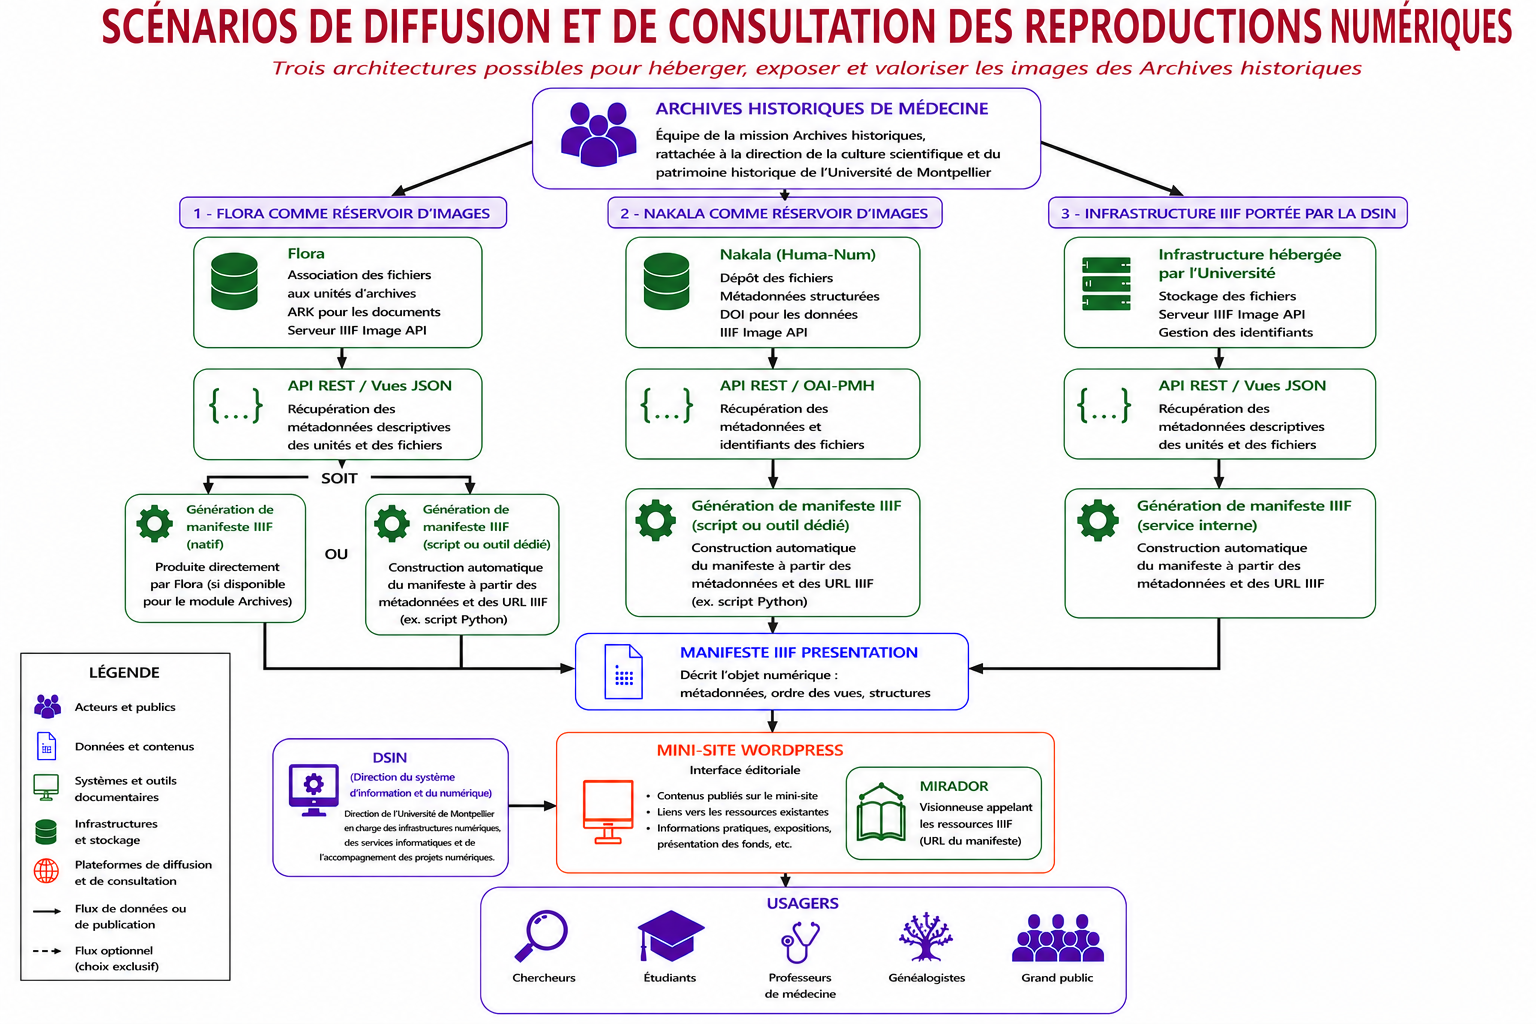
\includegraphics[
				width=\linewidth,
				height=1\textheight,
				keepaspectratio
				]{images/scenario2.png}
				\captionof{figure}{Scénarios envisagés pour l'hébergement, l'exposition et la consultation des reproductions numériques des Archives historiques}
				\label{fig:scenarios-diffusion-numerique}
			\end{minipage}%
		}
	\end{figure}
\end{landscape}

\chapter{Diffusion des archives historiques et gestion archivistique à l'échelle de l'Université}
\label{chap:systemes-information-archivistiques}
\chapitrecourt{Diffusion et gestion archivistique}

Les solutions examinées jusqu'ici répondent aux besoins immédiats de la Mission Archives historiques : produire et signaler les instruments de recherche, présenter les fonds, héberger les reproductions et en permettre la consultation. Leur articulation forme une architecture distribuée adaptée à un projet de diffusion, mais ne couvre pas l'ensemble des opérations archivistiques conduites à l'échelle de l'Université.

Le recours à un système d'information archivistique (\gls{sia}) relève d'une autre perspective : il vise à organiser dans un environnement métier commun la collecte, le traitement, la conservation et la communication des archives de l'établissement. Son étude conduit donc à changer d'échelle, depuis les dispositifs mobilisables par la Mission pour ses fonds historiques jusqu'à l'organisation de la fonction archives au niveau universitaire.


\section{Le \gls{sia} dans la gestion du cycle de vie des archives}
\label{sec:sia-changement-echelle}

\subsection{Les fonctions du \gls{sia}, de la collecte à la conservation définitive}

\paragraph{Un environnement commun pour les opérations archivistiques}

À la différence d'un \gls{cms}, d'un catalogue ou d'un portail documentaire, un \gls{sia} intervient dans les opérations quotidiennes du service. Selon son périmètre fonctionnel, il réunit la gestion des producteurs et des services versants, la collecte, les versements et les éliminations, le classement et la description, les localisations et le récolement, la communicabilité, les communications ainsi que la production d'instruments de recherche\footcite{Hamard2020}\footcite{MoalicMinnaert2023}.

Pour les archives courantes et intermédiaires, il assure principalement le suivi des producteurs et des versements, la localisation des articles, le contrôle des échéances, les éliminations et les communications. Pour les documents conservés définitivement, il prend en charge le classement hiérarchique, la description normalisée, la production des instruments de recherche et leur diffusion ou leur export.

\paragraph{La continuité des données au cours du cycle de vie}

L'intérêt du dispositif tient à la continuité des données entre ces différentes étapes. À l'issue de la durée d'utilité administrative, les documents éliminés sont retirés du système ; ceux qui doivent être conservés définitivement sont repris avec les informations déjà constituées sur leur producteur, leur provenance, leur versement, leur localisation et les traitements antérieurs. Le classement définitif complète ces données au lieu d'en imposer la reconstitution.

Cette continuité repose sur la constitution d'un \gls{referentiel} capable d'accompagner les documents au cours de leur cycle de vie. Elle prolonge l'évolution de l'informatisation archivistique, qui a progressivement étendu l'intervention de l'archiviste du traitement rétrospectif des fonds à la gestion des documents dès leur production\footcite{Hamard2020}.


\subsection{La séparation entre gestion métier et diffusion publique}

\paragraph{Des accès différenciés selon les utilisateurs et la communicabilité}

La continuité du traitement n'impose pas l'unicité des interfaces. Les solutions étudiées distinguent généralement un environnement professionnel de gestion d'une couche publique de diffusion : Mnesys Archives et Mnesys Expo, Ligéo Gestion et Ligéo Diffusion, ou encore Arkothèque Gestion et Arkothèque\footcite{MnesysLogiciels}\footcite{LigeoPresentation}\footcite{ArkothequePresentation}.

Cette séparation permet d'adapter les accès aux différents profils. Archivistes, services versants, agents de l'établissement et lecteurs extérieurs ne consultent pas les mêmes informations et n'accomplissent pas les mêmes opérations. Les habilitations doivent être articulées aux règles de communicabilité, aux restrictions particulières, aux éventuelles dérogations et aux conditions matérielles de consultation ; elles ne peuvent être réduites à une opposition entre contenus publiés et non publiés. Certaines solutions proposent ainsi des espaces distincts pour la collecte, le suivi des demandes et la gestion des communications\footcite{ArkothequeCollecte}\footcite{ArkothequeCommunication}.

Ces fonctions constituent l'un des points sur lesquels un \gls{sia} se distingue d'un logiciel documentaire plus généraliste. Les essais conduits par Sorbonne Université dans Flora ont ainsi révélé des difficultés à paramétrer assez finement les droits des administrateurs et des lecteurs et à traduire les règles de communicabilité dans l'interface de diffusion\footnote{Entretien avec Océane Valencia, responsable du Service des archives et du recueil des actes, Sorbonne Université, 6 juillet 2026.}. Sans remettre en cause les autres fonctions du logiciel, ce retour d'expérience montre les limites que peut rencontrer un outil qui n'est pas conçu prioritairement autour de la gestion du cycle de vie des archives. Dans un \gls{sia}, la communicabilité, les habilitations et les communications sont intégrées au traitement des unités documentaires et déterminent les conditions dans lesquelles celles-ci peuvent être rendues accessibles.

\paragraph{Le devenir du site éditorial selon le périmètre du \gls{sia}}

La présence d'un portail archivistique ne rend pas nécessairement inutile un site éditorial. Aux Archives municipales et métropolitaines de Montpellier, la base alimentée par Avenio donne accès depuis 2016 aux descriptions et aux ressources, tandis que le site créé en 2023 présente le service, ses activités et ses contenus de valorisation. Malgré leur rapprochement graphique, l'usager distingue encore difficilement le site institutionnel de la base ouverte par le bouton \enquote{Archives en ligne}\footnote{Entretien avec Claire Garcia, directrice adjointe et responsable de l'Unité Communication et Valorisation des Archives municipales et métropolitaines de Montpellier, 10 avril 2026.}. La coexistence de plusieurs interfaces suppose donc que leurs fonctions respectives soient clairement identifiables et que le parcours de l'une à l'autre demeure explicite.

À l'Université de Montpellier, la place du mini-site WordPress dépendrait ainsi du périmètre retenu pour un éventuel \gls{sia}. Limité à la gestion métier, celui-ci laisserait au mini-site ses fonctions de présentation de la Mission, d'information sur les modalités de consultation et de valorisation. L'acquisition d'une composante publique capable d'assurer à la fois la diffusion des instruments de recherche et des reproductions et l'accueil de contenus éditorialisés conduirait en revanche à réexaminer son maintien, afin d'éviter la duplication des informations et la multiplication des points d'accès.


\subsection{Le périmètre du \gls{sia} au regard des besoins et des moyens}

\paragraph{Des modules ajustés aux fonctions nécessaires}

Les solutions examinées pendant le stage --- principalement Mnesys, Ligéo, Avenio et Arkothèque --- organisent différemment la gestion, la diffusion et les échanges de données. Leur pertinence dépend des processus à prendre en charge, du volume et de l'état des données, du nombre d'utilisateurs, des habilitations nécessaires et des dispositifs de diffusion déjà en place.

Les retours d'expérience recueillis montrent que les établissements ne déploient pas nécessairement l'ensemble des composantes proposées. Après avoir comparé Flora, Mnesys, Ligéo, Avenio et Arkothèque, Sorbonne Université a retenu le seul module de gestion de Mnesys. Le portail n'a pas été acquis, les instruments de recherche étant déjà diffusés dans Calames et FranceArchives : le \gls{sia} est ainsi employé comme environnement métier, tandis que le \gls{signalement} et la consultation reposent sur des dispositifs extérieurs\footnote{Entretien avec Océane Valencia, responsable du Service des archives et du recueil des actes, Sorbonne Université, 6 juillet 2026.}.

À l'INALCO, deux ETP gèrent depuis 2025 environ 800 mètres linéaires avec Ligéo Gestion, principalement pour la collecte, les éliminations et les communications. Ligéo Diffusion n'a pas été acquis et les instruments restent proposés en PDF sur le site institutionnel ; Sciences Po utilise au contraire les deux composantes\footnote{Entretien avec Sarah Cadorel et Emma Bahous, INALCO, 15 juillet 2026.}\footcite{LigeoPresentation}. Arkothèque distingue pareillement la gestion des producteurs, des collectes, des versements, des éliminations et des communications de la publication des instruments et des ressources numériques\footcite{ArkothequeCollecte}\footcite{ArkothequeCommunication}\footcite{ArkothequePublication}. Ces configurations permettent d'ajuster le périmètre de l'outil métier aux besoins du service et aux dispositifs dont dispose déjà l'établissement.

Avenio offre une organisation différente. Aux Archives municipales et métropolitaines de Montpellier, les données métier alimentent directement la base publique et sa visionneuse\footnote{Entretien avec Claire Garcia, directrice adjointe et responsable de l'Unité Communication et Valorisation des Archives municipales et métropolitaines de Montpellier, 10 avril 2026.}. Cette comparaison reste indicative, l'échelle et les missions d'un service territorial différant de celles d'un établissement universitaire, mais elle confirme que l'articulation entre gestion et diffusion dépend du périmètre fonctionnel retenu plutôt que de l'existence d'un modèle unique de \gls{sia}.

\paragraph{Reprise des données, paramétrage et réorganisation du travail}

Le déploiement d'un \gls{sia} représente un investissement important. À Sorbonne Université, les quatre agents du service travaillaient depuis plusieurs mois à la préparation de Mnesys et avaient temporairement suspendu certaines opérations de collecte et de conseil afin de nettoyer et de restructurer les données\footnote{Entretien avec Océane Valencia, responsable du Service des archives et du recueil des actes, Sorbonne Université, 6 juillet 2026.}. À l'Université Paris Cité, la mise en œuvre, la migration et la formation auraient représenté environ une année de travail\footnote{Retour d'expérience de l'Université Paris Cité rapporté par Océane Valencia lors de l'entretien du 6 juillet 2026.}. Bien qu'indirect, ce retour fournit un ordre de grandeur de l'investissement organisationnel associé à une réinformatisation.

Une étude préalable devrait donc associer les futurs utilisateurs afin de formaliser les producteurs concernés, les procédures de collecte et de traitement, les données à reprendre, les règles de communicabilité, les habilitations, les échanges avec les autres applications et les besoins de diffusion. Le paramétrage ne se limite pas à transposer des pratiques existantes dans un logiciel : il les formalise et peut conduire à en reconfigurer certaines\footcite{MoalicMinnaert2023}.


\section{Une trajectoire de mise en œuvre pour les Archives historiques}
\label{sec:trajectoire-progressive}

L'étude des différents dispositifs permet de distinguer les opérations qui peuvent être engagées avec les moyens et les infrastructures actuellement disponibles de celles qui restent subordonnées à des choix techniques ou institutionnels. Le tableau~\ref{tab:comparaison-scenarios} rassemble les fonctions, les apports et les principales conditions de mise en œuvre des solutions examinées.

\begin{table}[htbp]
	\centering
	\tiny
	\setlength{\tabcolsep}{2pt}
	\renewcommand{\arraystretch}{1.15}
	\begin{tabularx}{\textwidth}{
			>{\raggedright\arraybackslash}p{1.75cm}
			>{\raggedright\arraybackslash}p{1.8cm}
			>{\raggedright\arraybackslash}p{2.15cm}
			>{\raggedright\arraybackslash}p{1.9cm}
			>{\raggedright\arraybackslash}X
			>{\raggedright\arraybackslash}X
		}
		\toprule
		\textbf{Dispositif} &
		\textbf{Fonction} &
		\textbf{Standards / échanges} &
		\textbf{Situation à l'UM} &
		\textbf{Intérêt} &
		\textbf{Conditions / limites} \\
		\midrule
		
		WordPress + \gls{mirador}
		& Médiation ; consultation des numérisations
		& \gls{iiif} Presentation
		& Mini-site déjà prototypé ; \gls{mirador} à intégrer
		& Interface éditoriale propre aux Archives ; réutilisation de ressources \gls{iiif} externes
		& Ne gère ni les descriptions archivistiques ni le stockage massif ; intégration de \gls{mirador} à réaliser \\
		
		\addlinespace
		
		SimplEAD + FranceArchives
		& \Gls{retroconversion} ; \gls{signalement} national
		& \gls{ead} 2002 ; \gls{oaipmh} côté FranceArchives
		& SimplEAD testé sur plusieurs instruments
		& Solution légère ; production d'un \gls{ead} valide sans déploiement d'un \gls{sia}
		& Sources maintenues localement ; nouvelle conversion après chaque modification ; identifiant du service à obtenir \\
		
		\addlinespace
		
		Calames
		& Production, maintenance et \gls{signalement} des instruments
		& \gls{ead} ; IdRef ; \gls{oaipmh}
		& Réseau déjà présent à l'UM
		& Production directe en \gls{ead} ; autorités partagées ; visibilité dans l'\gls{esr} et réutilisation des données
		& Intégration de la Mission à définir avec la référente et l'\Gls{abes} ; nouveaux déploiements suspendus pendant la refonte de Calames \\
		
		\addlinespace
		
		Flora
		& Gestion documentaire ; réservoir potentiel des reproductions
		& \gls{ark} ; \gls{api} \gls{json} ; \gls{iiif} Image
		& Déjà acquis et hébergé ; module Archives en cours de déploiement
		& Réutilisation d'une infrastructure institutionnelle ; absence d'un nouvel entrepôt
		& Export \gls{ead} testé non directement exploitable ; chaîne multi-images et \gls{iiif} Presentation non éprouvée \\
		
		\addlinespace
		
		Nakala
		& Hébergement et exposition des reproductions
		& \gls{doi} ; \gls{api} \gls{rest} ; \gls{oaipmh} ; \gls{iiif} Image
		& Non employé par la Mission
		& Entrepôt national indépendant des interfaces ; précédent Biblissima+ pour une chaîne \gls{iiif}
		& Nouvelle brique documentaire ; organisation des dépôts à définir ; \glspl{manifeste-iiif} Presentation à générer séparément \\
		
		\addlinespace
		
		Infrastructure \gls{dsin}
		& Hébergement ; services \gls{iiif} ; production des \glspl{manifeste-iiif}
		& \gls{iiif} Image / Presentation
		& Faisabilité évoquée ; architecture non définie
		& Maîtrise institutionnelle de la chaîne
		& Stockage, développement, sécurité et maintenance à dimensionner ; moyens non identifiés \\
		
		\addlinespace
		
		\gls{sia}
		& Gestion métier du cycle de vie
		& \gls{ead} et autres échanges selon la solution
		& Hypothèse à l'échelle de l'Université
		& Continuité des données entre archives courantes, intermédiaires et définitives
		& Projet institutionnel distinct : analyse des besoins, reprise des données, droits, paramétrage, formation et maintenance \\
		
		\bottomrule
	\end{tabularx}
	\caption{Fonctions, apports et conditions de mise en œuvre des dispositifs étudiés}
	\label{tab:comparaison-scenarios}
\end{table}


\subsection{Engager les opérations indépendantes des arbitrages techniques}

Plusieurs conditions demeurent ouvertes : l'identifiant nécessaire au versement dans FranceArchives, les modalités d'intégration à Calames, le devenir de cet environnement dans le cadre de sa refonte et le fonctionnement de la chaîne Flora--\gls{mirador}. Elles n'empêchent pas d'engager les travaux portant directement sur les données et les contenus.

Les instruments peuvent être harmonisés et repris progressivement ; ceux qui sont stabilisés peuvent être préparés dans SimplEAD ; la demande d'identification institutionnelle peut être adressée au \gls{siaf} ; les contenus et l'arborescence du mini-site peuvent être consolidés. La normalisation des producteurs, des cotes, des niveaux de description, des règles de communicabilité et des autorités prépare également leur utilisation dans des environnements ultérieurs. Le recours à l'\gls{ead} et à des \glspl{identifiant-perenne} permet de préserver leur capacité de circulation indépendamment de l'outil qui assure leur production ou leur publication à un moment donné.

Cette préparation intervient également dans la perspective d'une migration. Le passage des instruments de recherche de Harvard vers ArchivesSpace en fournit un exemple à une échelle beaucoup plus importante. Plus de 6\,000 instruments en \gls{ead}, représentant environ deux millions de composants archivistiques et issus de près de vingt années de pratiques d'encodage, devaient être repris dans le nouveau système. Malgré leur structuration dans un format commun, leurs variations internes et certaines données incompatibles avec le modèle cible auraient empêché l'import d'une part importante du corpus sans traitement préalable. La migration a reposé sur l'analyse des fichiers existants, l'identification de plusieurs dizaines de catégories de problèmes, leur transformation automatisée, puis des imports successifs dans un environnement de test contrôlés par les archivistes\footcite{MayoBowers2017}. Un format normalisé facilite donc la circulation des descriptions sans effacer l'hétérogénéité accumulée dans leurs modalités de production. L'harmonisation des instruments montpelliérains et la documentation des choix de structuration constituent à ce titre un travail préalable à leur exploitation présente comme à leurs éventuelles migrations futures.

Ces opérations doivent rester proportionnées aux priorités de la Mission, assurée par Sophie Dikoff et Emma Bertrand, et au calendrier de la demande de dérogation envisagée pour 2029. La connaissance et le classement des fonds, la révision ou la production des instruments de recherche, l'amélioration des conditions de conservation, l'organisation du service et la préparation du dossier demeurent prioritaires. Le développement de la diffusion numérique doit accompagner ces travaux sans mobiliser des moyens disproportionnés au regard des capacités actuelles du service.


\subsection{Éprouver les solutions disponibles avant de déployer de nouvelles infrastructures}

À court terme, SimplEAD permet de préparer le \gls{signalement} des instruments achevés, tandis que le mini-site assure leur médiation éditoriale. Pour les reproductions, Flora doit être testé en priorité puisque le logiciel est déjà acquis et en cours de déploiement à l'Université. L'essai devra vérifier la stabilité des identifiants et des URL, l'exposition des fichiers par \gls{iiif}, la production ou la génération extérieure des \glspl{manifeste-iiif} et leur restitution dans \gls{mirador}. Le recours à Nakala se justifierait si cette chaîne ne répond pas au besoin ; une infrastructure portée par la \gls{dsin} supposerait au préalable d'évaluer la charge de développement et de maintenance.

À moyen terme, Calames pourra être réexaminé avec la référente montpelliéraine et l'\Gls{abes}, lorsque les conditions d'intégration de la Mission et le calendrier de la refonte auront été précisés. Cette solution permettrait de remplacer la conversion ponctuelle des fichiers par une production et une maintenance partagées des instruments en \gls{ead}. Le projet Orion, qui renouvelle parallèlement le système de gestion des \glspl{metadonnees} et les outils de production de l'\Gls{abes}, devra également être suivi en raison de ses effets possibles sur l'écosystème documentaire de l'enseignement supérieur.

L'étude d'un \gls{sia} intervient à un horizon différent. Les retours d'expérience précédemment examinés montrent l'ampleur du travail de définition des processus, de reprise des données et de paramétrage qu'implique son déploiement. Son étude relève donc d'un projet institutionnel associant les différents acteurs de la fonction archives à l'échelle de l'Université, distinct des opérations de diffusion que la Mission peut engager à court et moyen terme.


\section*{Conclusion du chapitre et de la deuxième partie}
\phantomsection
\label{sec:conclusion-partie-ii}

L'étude, initialement centrée sur la création d'un portail propre aux Archives historiques, a conduit à dissocier plusieurs fonctions que la mise en ligne tendait d'abord à réunir : la médiation éditoriale, la production et le \gls{signalement} des descriptions, l'hébergement des reproductions et leur consultation. Les expérimentations menées montrent que leur prise en charge par des composants distincts permet de faire évoluer les dispositifs de diffusion sans imposer la reprise de l'ensemble des données. L'\gls{ead}, les \glspl{identifiant-perenne} et \gls{iiif} assurent à cet égard la circulation des descriptions et des reproductions entre des environnements susceptibles d'évoluer séparément.

Cette architecture distingue également deux échelles d'intervention. La Mission peut engager progressivement le \gls{signalement}, la médiation et la diffusion numérique de ses fonds à partir des infrastructures disponibles, tandis que la continuité de leur gestion avec celle des archives courantes et intermédiaires relève d'un éventuel \gls{sia} conçu à l'échelle de l'établissement. Les travaux entrepris sur les fonds historiques répondent ainsi aux besoins présents sans présumer de l'environnement métier qui pourrait être retenu ultérieurement.

La circulation des descriptions et des reproductions ouvre enfin la possibilité de rapprocher les Archives historiques des autres ensembles documentaires auxquels leur histoire les relie. Les personnes, institutions, enseignements et pratiques documentés par les fonds ont laissé d'autres traces dans les bibliothèques et les collections scientifiques de l'Université, comme dans les établissements patrimoniaux montpelliérains ; les données produites à partir des archives peuvent également rejoindre des réseaux documentaires et des infrastructures de recherche dépassant l'échelle locale. Ces relations entre collections, institutions et données constituent dès lors le prolongement de la réflexion sur leur diffusion.